\documentclass[acmsmall,review,anonymous,nonacm]{acmart}
\usepackage{mathpartir}
\usepackage{cleveref}
\usepackage{listings}
\usepackage{svg}
\usepackage{float}
\usepackage{caption}
\usepackage{subcaption}
\usepackage{graphicx}
\usepackage{amsmath}
\usepackage{multirow} 
\usepackage{tikz}
\usepackage{listings}
\usepackage{xcolor}
\usepackage{booktabs} 
\usepackage{arydshln}
\usepackage[table]{xcolor}
\usepackage[dvipsnames]{xcolor}  
\usepackage{siunitx}
\usepackage{multirow}
\usepackage{pifont}
\usepackage{calc} 
%\newcommand{\cmark}{\textcolor{green}{\ding{51}}}
\usepackage{wrapfig}             % for wrapfigure
\usepackage[export]{adjustbox}   % for trim/clip keys on includegraphics
\usepackage[T1]{fontenc}
\usepackage{tcolorbox}           % for colored boxes
\newcommand{\cmark}{\checkmark}
%\definecolor{brightbrown}{RGB}{245,237,205}%{205,133,63}
%\colorlet{darksand}{Tan!50!black}
%\definecolor{strongyellow}{RGB}{255,220,0}
\definecolor{brightyellow}{RGB}{255,247,192}%{255,255,102}
\definecolor{lightchacki}{RGB}{245,237,205}%{235,220,187}



% Define darkorange via RGB or HTML:
\definecolor{darkorange}{RGB}{255,140,0}

\newcommand{\xmark}{\textcolor{red}{\ding{55}}}
\usetikzlibrary{shapes.geometric,positioning,arrows} 
\definecolor{headerbg}{RGB}{220,230,241}

\newcommand{\Pre}{\mathit{Pre}}
\newcommand{\Post}{\mathit{Post}}

% ----- Macros -----

% Tool name macro (styled like typical POPL papers)
\newcommand{\toolname}{\textsc{Ser}}

\newcommand{\guy}[1]{\textcolor{green!50!black}{G: #1}}
\newcommand{\jules}[1]{\textcolor{red!50!black}{J: #1}}
\newcommand{\markb}[1]{\textcolor{blue!50!black}{M: #1}}
\newcommand{\todo}[1]{\textcolor{gray}{TODO: #1}}


\newcommand{\grammartag}[1]{\qquad\qquad\emph{(#1)}}


% Define macros for keywords
\newcommand{\kw}[1]{\textbf{#1}}
\newcommand{\nondet}{\kw{?}}
\newcommand{\ifkw}{\kw{if}}
\newcommand{\elsekw}{\kw{else}}
\newcommand{\whilekw}{\kw{while}}
\newcommand{\yieldkw}{\kw{yield}}
\newcommand{\requestkw}{\kw{request}}

\newcommand{\sat}{\texttt{SAT}}
\newcommand{\unsat}{\texttt{UNSAT}}

\newcommand{\Parikh}{\mathsf{Parikh}}

\newcommand{\greencmark}{\textcolor{green}{\ding{51}}}

\lstdefinelanguage{CustomPseudoCode}{
	morekeywords={request, yield, return, if, else, while, and, or},
	morecomment=[l]{//},
	morestring=[b]",
	sensitive=true
}

\lstset{
	language=CustomPseudoCode,
	basicstyle=\ttfamily\small,
	keywordstyle=\color{blue}\bfseries,
	commentstyle=\color{gray}\itshape,
	stringstyle=\color{orange},
	numbers=left,
	numberstyle=\tiny,
	stepnumber=1,
	numbersep=5pt,
	backgroundcolor=\color{white},
	frame=single,
	rulecolor=\color{black},
	tabsize=2,
	captionpos=b,
	breaklines=true,
	breakatwhitespace=false,
	showstringspaces=false,
	escapeinside={(*@}{@*)},  % used for coloring "?" below
}


% ----- Main paper -----

\title{When One Message Tells the Whole Story:\\ Deciding Serializability in Network Systems}
\author{Author Name}
\affiliation{
  \institution{Institution Name}
  \city{City}
  \state{State}
  \country{Country}
}
\email{author@institution.edu}

\settopmatter{printfolios=false,printccs=false,printacmref=false}
\renewcommand\footnotetextcopyrightpermission[1]{} % removes footnote with DOI
% \renewcommand{\keywords}[1]{}  % removes "Additional keywords and phrases"
% \renewcommand{\acmSubmissionID}[1]{} % removes SUBMISSION ID
\let\oldmaketitle\maketitle
\renewcommand{\maketitle}{
  \oldmaketitle
  \pagestyle{plain}  % empty headers and footers on all pages
  \thispagestyle{plain}  % empty header and footer on the first page
}

% Make paragraph headings bold
\makeatletter
\renewcommand\paragraph{\@startsection{paragraph}{4}{\z@}%
  {1.5ex \@plus1ex \@minus.2ex}%
  {-1em}%
  {\normalfont\normalsize\bfseries}}
\makeatother

% Redefine sections to display with § symbol
\crefformat{section}{\S#2#1#3}
\Crefformat{section}{\S#2#1#3}

% Ensure subsections/subsubsections behave the same way (optional)
\crefformat{subsection}{\S#2#1#3}
\Crefformat{subsection}{\S#2#1#3}
\crefformat{subsubsection}{\S#2#1#3}
\Crefformat{subsubsection}{\S#2#1#3}

% 1) create a new length
\newlength{\subfigheight}

% 2) measure the height of (d) once the document begins
\AtBeginDocument{%
	\settoheight{\subfigheight}{%
		\includegraphics[width=0.23\textwidth]{plots/bidirectional_pruning_step_d_updated_2.pdf}%
	}%
}

\begin{document}

\begin{abstract}
	We introduce the \toolname{} modeling language and toolchain for automatically verifying or disproving serializability of concurrent programs, i.e., whether every concurrent execution of the program is equivalent to some serial execution. \toolname{} programs are suitably restricted to make this problem decidable, while still allowing for an unbounded number of concurrent threads of execution, each potentially running for an unbounded number of steps.
	Prior work has shown theoretical decidability of this problem via reductions to Petri-net reachability, but \toolname{} is the first to provide an end-to-end decision procedure and toolchain that proves serializability (generating a proof certificate) or non-serializability (generating a counterexample trace).
	We demonstrate this on various example models of SDN scenarios, stateful firewalls, BGP routers, online shopping backends, and more.
	Our verifier operates by translating network system programs into Petri nets, but this is not enough: we introduce various techniques, such as Petri net pruning, semilinear-set compression, and Presburger-formula manipulation.
	Our solver is thus able to automatically prove serializability or prove non-serializability for interesting examples, despite the theoretical hardness of the problem.
\end{abstract}

%\begin{abstract}
%	\input{sections/0_abstract}
%\end{abstract}

\maketitle

% \keywords{programming languages, static analysis, verification}

\section{Introduction}
\label{sec:introduction}

\todo{Introduction goes here.}

\todo{We motivate the problem of deciding serializability in programmable networks.}

\todo{We talk about some related work if relevant.}

\todo{We show that it's interesting with an example.}

\todo{We describe our main results.}

\paragraph{Contributions:}
\begin{itemize}
    \item Novel notion of serializability (``atomicity'') applicable to network systems
    \item Decidability results (1 main theorem: \textbf{automatically proving unbounded serializability}, 2 extra theorems: ser=ser decidable, ser=int undecidable)
    \item Implementation of decision procedure
    \item Advances in semilinear sets, Petri net reachability heuristics that makes the decision procedure work
\end{itemize}
%\newpage


\section{Tour / examples}
\label{sec:tour}

Next, we will walk through a series of examples, in varying level of complexity. Each example will demonstrate different aspects of serializable vs non-serializable programs.
%
The first examples are relatively basic, while the last examples have higher complexity and are motivated by real word problems, e.g., BGP routing policy updates.
%
Global variables are depicted with upper-case characters, while local variables (per each request) are depicted with lower-case ones.
%
Unless explicitly state otherwise, all global and local variables are initialized to 0.
%
The ``\textit{?}'' symbol depicts a nondeterministic choice between ``0'' and ``1''. All other constructs (\textit{while}, \textit{yield} \textit{if}) have their common interpretation.

\guy{Is the above paragraph clear?}

\subsection{Example 1}

%\subsubsection{Example 1}

We start with a basic example, describing a single request {\color{ForestGreen}$\blacklozenge_\text{A}$}, a single local variable (``x'') per each request; and a single global variable (``FLAG'') shared among all in-flight requests. 
%
In Listing~\ref{lst:BasicSer} an in-flight request assigns to x the value of FLAG (hence, initially, [$x:=0$]). Then, the request non-deterministically chooses whether to yield, or to flip the value of $x$. Subsequently, FLAG is assigned 1 and the value of x is returned as the response to request {\color{ForestGreen}$\blacklozenge_\text{A}$}. 
%
Note that the presence of the \textit{else} branch renders the program serializable, as intuitively, the returned value of x does not depend on the assignment of FLAG.
%
However, this changes in  Listing~\ref{lst:BasicNonSer}. In which case there is no ``else'' branch and x is always assigned the value of FLAG.
%
It is straightforward to see that this update makes the program non-serializable. Any serial execution will afford the first request {\color{ForestGreen}$\blacklozenge_\text{A}$} the matching returned response {\color{red}$\blacklozenge_0$} (as $[x:=FLAG]$, which is initially 0). As the first request also assigns $[FLAG:=1]$ before exiting, any subsequent execution will assign $[x:=1]$ and hence return the response {\color{red}$\blacklozenge_1$}. Differently put, for any serial execution with i requests --- we have exactly one (first) request/response pair {\color{ForestGreen}$\blacklozenge_\text{A}$}/{\color{red}$\blacklozenge_0$}, and $(i-1)$ pairs of {\color{ForestGreen}$\blacklozenge_\text{A}$}/{\color{red}$\blacklozenge_1$}.
%
However, given that the first request can also \textit{yield}, it is possible for another request to subsequently run the program after the first request yields and before it returns. This, in turn, will allow two requests to have $[x=0]$, and hence, any number of arbitrary requests can have multiple {\color{ForestGreen}$\blacklozenge_\text{A}$}/{\color{red}$\blacklozenge_0$} pairs. Thus, Listing~\ref{lst:BasicNonSer} is not serializable.




%\vspace{2em}
%example - 2

% Second row
\noindent
\begin{minipage}[t]{0.45\textwidth}
	\begin{lstlisting}[caption={Serializable},
		label={lst:BasicSer}]
	request A: 
		x := FLAG
		
		if (?):
			yield
		else:
			x := 1 - x
		
		FLAG := 1
		return x
	\end{lstlisting}
\end{minipage}
\hfill
\begin{minipage}[t]{0.45\textwidth}
	\begin{lstlisting}[caption={Not serializable: {(A,0),(A,0)}},
	label={lst:BasicNonSer}]
			request A: 
			    x := FLAG 
			
			    if (?): 
			        yield
			    // no else
			
			
			    FLAG := 1 
			    return x
		\end{lstlisting}
\end{minipage}%

\subsection{Example 2}

%\subsubsection{Example 2}
The following program pairs have a single global variable ``X'', and two requests --- {\color{ForestGreen}$\blacklozenge_\text{incr}$} which increments X by 1, and {\color{ForestGreen}$\blacklozenge_\text{decr}$} which decrements X by 1. Both program have while loops which guarantee that X will always be assigned a value between 0 to 3, otherwise the while loop will yield an infinitum. Both requests return the value of X after updating it.
%
In the first case, Listing~\ref{lst:FredSer} presents a serializable execution, due to the absence of any yield between the increment/decrement of X, and its return. Equivalently, in each of the requests, the update of X and the returned value can be thought of as \textit{a single atomic execution}.
%
However, in Listing~\ref{lst:FredNonSer},we add an additional yield (and a local variable ``y''), occurring in each of the requests, between the update of X and it's return.
%
This updates allows request of the same type to update X to the same value --- something that is not possible in any serial execution. 

%\vspace{2em}
%\newpage
%example - 3

% Third row
\noindent
\begin{minipage}[t]{0.45\textwidth}
	\begin{lstlisting}[caption={Fred (serializable)},
		label={lst:FredSer}]
			request incr: 
			    while (X == 3):
			        yield
			        
			        
			    X := X + 1
				  return X		
			
			request decr: 
			    while (X == 0): 
			        yield
			        
			        
			    X := X - 1
				  return X
		\end{lstlisting}
\end{minipage}
\hfill
\begin{minipage}[t]{0.45\textwidth}
	\begin{lstlisting}[caption={Fred2 (not serializable)},
		label={lst:FredNonSer}]
			request incr:
			    while (X == 3):
			        yield
			    y := X
			    yield
			    X := y + 1
		      return X		
			
			request decr: 
			    while (X == 0):
			        yield
			    y := X
			    yield
			    X := y - 1
		      return X
		\end{lstlisting}
\end{minipage}
	
\subsection{Example 3}
%\subsubsection{Example 3}	
%\todo{continue}	
%example - 6

The next pair of examples cover a setting in which there is a single global variable (X) and a single local variable per each in-flight request. The {\color{ForestGreen}$\blacklozenge_\text{flip}$} requests flips the bit of the single initial variable X (initialized to 0); the {\color{ForestGreen}$\blacklozenge_\text{main}$} request attempts to decrement i five times.
%
It is straightforward to observe that the program in Listing~\ref{lst:ComplexWhileSer} is trivially serializable, as there are no yields.
%
However, by adding the two yields and updating the program (see Listing~\ref{lst:ComplexWhileNonSer}) it becomes non-serializable. This can be observed as follows --- given a single in-flight request, the value of X is either 0 or 1, and hence, exactly one of the while loops will run indefinitely. Thus, any serializable execution will result into a set without any {\color{ForestGreen}$\blacklozenge_\text{main}$}/{\color{red}$\blacklozenge_1$} pairs, but rather only, perhaps terminating {\color{ForestGreen}$\blacklozenge_\text{flip}$} requests.
%
However, given at least $i=5$ interleaving of in-flight {\color{ForestGreen}$\blacklozenge_\text{flip}$} requests, it is possible for a {\color{ForestGreen}$\blacklozenge_\text{main}$} request to terminate and bypass all while loops, something that cannot occur in serializable executions.


% Second row
\noindent
\begin{minipage}[t]{0.45\textwidth}
	\begin{lstlisting}[caption={Complex while (serializable)},
		label={lst:ComplexWhileSer}]
		    request flip: 
		        X := 1 - X 
		    
		    request main:
		        i := 5
		        while (i > 0):
		            while (X == 0):
		                pass
		            while (X == 1):
		                pass
		            i := i - 1
		        
		        return 1       
				\end{lstlisting}
\end{minipage}%
\hfill
\begin{minipage}[t]{0.45\textwidth}
	\begin{lstlisting}[caption={Complex while with yields (not serializable)},
		label={lst:ComplexWhileNonSer}]
		    request flip: 
		        X := 1 - X 
		
		    request main:
		        i := 5
		        while (i > 0):
		            while (X == 0):
		                yield
		            while (X == 1):
		                yield
		            i := i - 1
		
		        return 1        
					\end{lstlisting}
\end{minipage}
	
	
	
\subsection{Example 4}
%\subsubsection{Example 4: Banking System}

The next example emulates a simple banking system, as motivated by Chandy and Lamport's seminal paper~\cite{ChLa85}. The system operates on two accounts of the same user --- denoted with the global variables $A$ and $B$, and initialized to have $100\$$ and $50\$$ respectively. 
%
Each {\color{ForestGreen}$\blacklozenge_\text{transfer}$} request allocates $50\$$ from account $A$ to account $B$, and every {\color{ForestGreen}$\blacklozenge_\text{interest}$} request adds $t\%$ interest to each account. For simplicity, and without loss of generality, we chose $t=100\%$, hence doubling the funds in each account, per each such request. We also note that for simplicity we depict two accounts ($A$ and $B$), although this example is valid for any number of accounts.
%
Both requests return the sum of final client funds in both the accounts.  
%
Listing~\ref{lst:BankSer} depicts a serializable version of this banking system (without any yields), while Listing~\ref{lst:BankNonSer} includes yields in each of the requests, between the adjustment of accounts $A$ and $B$ (we note that this also represents real world systems in which the account can be sharded and partitioned across different nodes).
%


\noindent
\begin{minipage}[t]{0.45\textwidth}
	\begin{lstlisting}[caption={bank (serializable)},
		label={lst:BankSer}]
	    // initialize accounts
	    A := 100
	    B := 50
	    
	    request transfer: 
	        // transfer 50$
	        A := A - 50
	        // no yield
	        B := B + 50
	        return A + B
				
	    request interest: 
	        // add a 100% interest
	        A := A + A
	        // no yield
	        B := B + B
	        return A + B	      		        
			\end{lstlisting}
\end{minipage}
\hfill
\begin{minipage}[t]{0.45\textwidth}
	\begin{lstlisting}[caption={bank with yields (non serializable)},
		label={lst:BankNonSer}]
	    // initialize accounts
	    A := 100
	    B := 50
			
	    request transfer: 
	        // transfer 50$
	        A := A - 50
	        yield
	        B := B + 50
	        return A + B
	
	    request interest: 
	        // add a 100% interest
	        A := A + A
	        yield
	        B := B + B
	        return A + B	      		        
		\end{lstlisting}
\end{minipage}
	

Interestingly, in this setting, serializability also corresponds to correctness invariants pertaining to the program. Specifically, in every serializable execution, it holds that for $A_{\textit{before}},B_{\textit{before}}$ marking the funds before running a single {\color{ForestGreen}$\blacklozenge_\text{interest}$} request, and any number of {\color{ForestGreen}$\blacklozenge_\text{transfer}$} requests (and $A_{\textit{after}},B_{\textit{after}}$ marking the corresponding state after those requests), then:
\[
\bigl(A_{\mathit{after}} + B_{\mathit{after}}\bigr)
= (1 + t\%)\,\bigl(A_{\mathit{before}} + B_{\mathit{before}}\bigr).
\]

This invariant always holds for any such serial execution, while having the specific division \textit{between} accounts $A$ and $B$ depending on the actual order of the serial execution.
%
However, this correctness invariant does not hold for non serializable executions. For example, in a setting in which there is a single {\color{ForestGreen}$\blacklozenge_\text{transfer}$} request, which deduces $50\%$ from account $A$, and then yields (resulting to a temporary state in which $[A=50\$,B=50\$]$); subsequently followed by an  {\color{ForestGreen}$\blacklozenge_\text{interest}$} request which runs until completion, in which case  $[A=100\$,B=100\$]$, and then, the remainder of the yielded {\color{ForestGreen}$\blacklozenge_\text{transfer}$} request is executed, resulting finally to $[A=100\$, B=150\$]$.  This result in $50\$$ ``missing'' from our system, due to this non serializable behavior.
%
As mentioned, a serial execution of a these two request will always result to 
$A+B=2\cdot (100\$+50\$)=300\$$, with either a final state of $[A=150\$, B=150\$]$ or $[A=100\$, B=200\$]$, depending on the scheduled serializable order.




%\newpage
\subsection{Example 5}

The following example motivates our routing‐policy programs in software‐defined networking (SDN). In SDN, switches not only forward packets but can also be programmed in domain‐specific languages (e.g., P4). At runtime, a centralized controller node can adjust the global network control policy. The controller can also periodically send control packets to each switch, causing it to adopt its updated routing as dictated by the updates.
%
An instance of a simple network with two competing policies is shown in Fig.~\ref{fig:BgpRoutingPolicies}. This network consists of four nodes (numbered 0 through 3), with the two middle nodes --- node 1 (labeled \textit{WEST}) and node 2 (labeled \textit{EAST}), serving as ingress points from where traffic may nondeterministically enter the network. The controller selects one of two policies: a \textcolor{NavyBlue}{blue} policy, which routes traffic from West to East, or a \textcolor{darkorange}{orange} policy, which routes it in the opposite direction.


%// [WEST, switch 1] ---> [EAST, switch 2] ---> [out, switch 3] 
%else:
%B := 0 // red/orange policy
%// [out, switch 0] <--- [WEST, switch 1] <--- [EAST, switch 2] 

\begin{wrapfigure}{r}{0.45\textwidth}  % “r” = wrap on the right, width = 45% of line
	\centering
	\includegraphics[
	width=\linewidth,
	trim=10 15 15 5,   % {left bottom right top} — tweak as needed
	clip
	]{plots/east_west_routing_updated_colors.pdf}
	\caption{Routing policy in example 5.}
	\label{fig:BgpRoutingPolicies}
\end{wrapfigure}

%\begin{figure}[H]
%	\centering
%	\includegraphics[width=0.5\linewidth]{plots/east_west_routing_updated_colors.pdf}
%	\caption{Routing policy in example 5.}
%	\label{fig:BgpRoutingPolicies}
%\end{figure}

This SDN-controlled routing policy is realized in the pseudo code in Listing~\ref{lst:BgpNonSerializable}.
%
The program includes a single global variable $B$, indicating if the current routing policy is the  \textcolor{NavyBlue}{blue} policy ($[B=1]$) or the \textcolor{darkorange}{orange} policy ($[B=0]$).
%
The program has three types of requests:
%\begin{itemize}
%	
%	\item
	(i)
	{\color{ForestGreen}$\blacklozenge_\text{policy update}$}:
%	\textit{policy update}:
 represents a controller  update, which nondeterministically decides whether to update the policy (i.e., flip the value of  variable $G$) or not;
%	
%		\item
(ii)
	{\color{ForestGreen}$\blacklozenge_\text{route\_from\_west}$}:
	 this request represents a packet entering the network from the \textit{WEST} node (node 1); and 
%	
%		\item
(iii)
{\color{ForestGreen}$\blacklozenge_\text{route\_from\_east}$}: this request represents a packet entering the network from the \textit{EAST} node (node 2).
	
%\end{itemize}

Each of the routing requests represents a single packet entering the network. The request includes a local \textit{current} variable representing the index of the current node visited. This variable is initialized as the ingress node value, and updated to emulate the chosen routing path. There is also a \textit{visited\_east} variable (or a \textit{visited\_west} variable, depending on the request in question).
%
The return value of the {\color{ForestGreen}$\blacklozenge_\text{route\_from\_west}$} requests is the sum \textit{(current+current+visited\_east)}. This is an identifier encoding all possible \textit{(current\_switch, visited\_east)} pairs.
%
The program is not serializable, as witnessed by an interleaving that can give rise to final return value of \textit{(current+current+visited\_east)=1} (due to \textit{current=0} and \textit{visited\_east=1}). This represents a routing cycle in the network, which is possible only when updated the routing policy after a request has already been routed based on the previous policy.
Legal, acyclic routes of this request have either a return value of 0 (in the case of [\textit{current=0}, \textit{visited\_east=0}]) or 7 (in the case of [\textit{current=3}, \textit{visited\_east=1}]).
Potential routing cycles can also be observed via non serializable executions also for the  {\color{ForestGreen}$\blacklozenge_\text{route\_from\_east}$} requests.



\begin{minipage}[t]{1.0\textwidth}
	\begin{lstlisting}[caption={BGP (non serializable --- cycles can appear)},label={lst:BgpNonSerializable}]
	    // initialize accounts
	    B := 0
	    
	    request policy_update:
	    if (?):
	        B := 1  // blue policy 
	    else:
	        B := 0 // orange policy
			
	    request route_from_west:
	        visited_east := 0
	        current := 1
	        while (current == 2) or (current == 3): // still routing        
	            if (current == 1): // west (switch 1)
	                if (B == 1): // blue policy
	                    current := 2
	                else: // orange policy
	                    current := 1
	            if (current == 2): // east (switch 2)
	                visited_east := 1
	                if (B == 1): // blue policy
	                    current := 3
	                else: // orange policy
	                    current := 1
	 
	            yield
			
	        return current + current + visited_east
	        
	    request route_from_east:
	        ... // dual case     		        
		\end{lstlisting}
\end{minipage}






\subsection{Example 6}

We add an additional example for network monitoring and \textit{snapshot isolation} in Appendix~\ref{}.
%\guy{suddenly I'm not so sure about this example. It is indeed sound but maybe a bit silly?}


The next program is motivated by system monitoring.
The system has two nodes (represented by the global variables $N_1$ and $N_2$) which monitor ongoing traffic in the network, and are originally both active (as indicated by their initial values [$N_1=1,N_2=1$]).
%
The {\color{ForestGreen}$\blacklozenge_\text{main}$} request takes a ``snapshot'' of the system, i.e., locally records the current activation status of each of the two nodes.
%
Subsequently, in the first request, and any future ones in which both nodes are active, each in-flight request thread  non-deterministically decides which of the two nodes to deactivate, i.e. set [$N_i:=0$]. This policy is consistent with real-world settings for maintaining overall energy efficiency.
%
The {\color{ForestGreen}$\blacklozenge_\text{main}$} request eventually returns the current sum of active nodes in the system.
%
In order for the system to emulate multiple iterations, our setting also includes two additional requests, {\color{ForestGreen}$\blacklozenge_\text{activate\_n1}$},{\color{ForestGreen}$\blacklozenge_\text{activate\_n2}$} which activate the nodes $N_1$ and $N_2$, respectively.
%
We note that the program is non-serializable due to the yield operation that appears immediately after the recording (snapshot) of the node activity. One such example for a non-serializable behavior occurs when two {\color{ForestGreen}$\blacklozenge_\text{main}$} requests record two active monitor nodes and yield; Then, having each request turn off the complement node. As a result of each request operating based on its isolated ``snapshot'' of the initial global state, both monitor nodes can be turned off and we can attain a request with {\color{ForestGreen}$\blacklozenge_\text{main}$}/{\color{red}$\blacklozenge_0$} (for [$N_1+N_2=0+0=0$]).
%
We note that in any serializable execution, no two {\color{ForestGreen}$\blacklozenge_\text{main}$} requests can record both monitors as active, and hence, they cannot both have an interleaving in which each separate monitor is deactivated (hence, a response of {\color{red}$\blacklozenge_0$} is unattainable in serializable executions).




\begin{minipage}[t]{1.0\textwidth}
	\begin{lstlisting}[caption={Snapshot-based monitor deactivation (not serializable, as it can return a sum of 0 active monitors)}]
			// initialize both monitors to be active
			N_1_ACTIVE := 1
			N_2_ACTIVE := 1
			
			request main:
				// take snapshot
				n_1_active_snapshot := N_1_ACTIVE
				n_2_active_snapshot := N_2_ACTIVE
				yield
				
				if (n_1_active_snapshot == 1) and (n_2_active_snapshot == 1):
				// if both nodes active --- choose which one to deactivate 
					if (?): 
						  N_1_ACTIVE := 0
					else:
						  N_2_ACTIVE := 0
					
				return N_1_ACTIVE + N_2_ACTIVE  // total active nodes
				
			
			request activate_n1:
				    N_1_ACTIVE := 1
			
			request activate_n2:
				    N_2_ACTIVE := 1
			
			
		\end{lstlisting}
\end{minipage}

%only 0 in non-serializable runs!

%\todo{start}

%/snapshot_isolation_directly_as_NS_with_yields

%\begin{figure}[h]
%	\centering
%	\includegraphics[width=1.0\linewidth]{plots/snapshot\_isolation\_JSON\_with\_yields.pdf}
%	\caption{Snapshot Isolation with Yields.}
%	\label{fig:snapshotIsolationJsonWithYields}
%\end{figure}
%
%
%
%%/snapshot_isolation_directly_as_NS_without_yields
%
%\begin{figure}[h]
%	\centering
%	\includegraphics[width=1.0\linewidth]{plots/snapshot\_isolation\_JSON\_without\_yields.pdf}
%	\caption{Snapshot Isolation without Yields.}
%	\label{fig:snapshotIsolationJsonWithoutYields}
%\end{figure}


%\todo{maybe we have: (1) a copy of the global automaton; (2) a copy of the local automaton (with yields) with coloring of edges that don't exist in the one without yields}


%\begin{figure}[h]
%	\centering
%	\includegraphics[width=0.65\linewidth]{plots/BgpColoredRouting.pdf}
%	\caption{Routing policy in example 7.}
%	\label{fig:pdfimage}
%\end{figure}

%\newpage
%
%
%example – 8
%
%\noindent
%\begin{minipage}[t]{0.45\textwidth}
%	\begin{lstlisting}[caption={foo (serializable)}]
%	request foo: 
%	    if (?):
%	        X := (X + 2) % 3 
%	        // no yield
%	        return X
%	
%	    else:
%	        X := (X + 1) % 3
%	        // no yield
%	        return X
%		\end{lstlisting}
%\end{minipage}
%\hfill
%\begin{minipage}[t]{0.45\textwidth}
%\begin{lstlisting}[caption={foo (non serializable)}]
%request foo: 
%     if (?):
%         X := (X + 2) % 3 
%         yield
%         return X
%
%     else:
%         X := (X + 1) % 3
%         yield
%         return X
%	\end{lstlisting}
%\end{minipage}
%
%One output that is attainable only via non-serializable executions is 
%\[
%\{(foo,1),(foo,1),(foo,1),(foo,3)\}
%\]
%
%
%%\newpage
%
%
%example – 9
%
%\noindent
%\begin{minipage}[t]{0.45\textwidth}
%	\begin{lstlisting}[caption={foo (serializable)}]
%request foo:
%    if(STOP == 0):
%        X := (X + 1) % 4
%
%    yield
%
%    if(STOP == 0):
%        X := (X + 1) % 4
%
%        STOP := ?
%        
%        if(STOP == 1):
%	        return X
%        return 0
%	\end{lstlisting}
%\end{minipage}
%\hfill
%\begin{minipage}[t]{0.45\textwidth}
%	\begin{lstlisting}[caption={foo (non serializable)}]
%request foo:
%    if(STOP == 0):
%        X := (X + 1) % 4
%
%    yield
%
%    if(STOP == 0):
%        X := (X + 2) % 4
%
%        STOP := ?
%        
%        if(STOP == 1):
%	        return X
%        return 0
%	\end{lstlisting}
%\end{minipage}



\newpage

\section{Problem Definition}
\label{sec:problem-definition}

\newcommand{\grammartag}[1]{\qquad\qquad\emph{(#1)}}
\begin{figure}[t]
    \begin{align*}
    \mathbf{Expression}\quad e ::= &&& \\
       | & \quad 0 \mid 1 \mid 2 \mid \ldots                                && \grammartag{Numeric constants} \\
       | & \quad \nondet                                 && \grammartag{Nondeterministic value: 0 or 1}\\
       | & \quad x := e                            && \grammartag{Write to local packet field} \\
       | & \quad x                                 && \grammartag{Read from local packet field} \\
       | & \quad X := e                            && \grammartag{Write to global switch variable} \\
       | & \quad X                                 && \grammartag{Read from global switch variable} \\
       | & \quad e_1 == e_2                        && \grammartag{Equality test} \\
       | & \quad e_1 ; e_2                         && \grammartag{Sequencing} \\
       | & \quad \ifkw(e_1)\{\ e_2\ \}\elsekw\{\ e_3\ \} && \grammartag{Conditional} \\
       | & \quad \whilekw(e_1)\{\ e_2\ \}              && \grammartag{While loop} \\
       | & \quad \yieldkw                      && \grammartag{Yields to scheduler}\\[1em]
    \mathbf{Program}\quad p ::=
        & \quad \requestkw\ name_1\ \{\ e_1\ \}&&\grammartag{Set of request handlers}\\[-0.5em]
        & \quad \qquad \vdots &&\\
        & \quad \requestkw\ name_n\ \{\ e_n\ \}\ 
    \end{align*}
    \caption{Syntax of expressians and programs}
    \label{fig:syntax}
\end{figure}
    
A Network System $\mathcal{N}$ is a tuple $(G, L, \mathit{Req}, \mathit{Res}, g_0, \delta, \mathit{req}, \mathit{resp})$ where:
\begin{itemize}
\item $G$ is a set of global states representing switch state
\item $L$ is a set of local states representing packet contents
\item $\mathit{Req}$ is a set of request events
\item $\mathit{Res}$ is a set of response events
\item $g_0 \in G$ is the initial global state
\item $\mathit{req} \subseteq \mathit{Req} \times L$ is a request transition relation, which describes which requests turn into which packets
\item $\mathit{resp} \subseteq L \times \mathit{Res}$ is a response transition relation, which describes which packets turn into which responses
\item $\delta \subseteq (G \times L) \times (G \times L)$ is a transition relation for packet processing, which describes an atomic step of packet processing that may change the global state.
\end{itemize}

\begin{figure}[t]
    \centering
    \renewcommand{\arraystretch}{1.6}
    \[
    \begin{array}{c}
    \textbf{States and Transitions:}
    \\
    \quad
    \text{A (global) \emph{network state} is a triple }(g,\mathcal{P},M)\text{ where:}
    \\
    \quad
    g \in G \text{ is the current global switch state,}
    \\
    \quad
    \mathcal{P} \in \text{Multiset}(L \times \mathit{Req}) \text{ is a multiset of in-flight packets,}
    \\
    \quad
    M \in \text{Multiset}(\mathit{Req} \times \mathit{Res}) \text{ is a multiset of request--response pairs already completed.}
    \end{array}
    \]

    \[
    \begin{array}{c}
    \textbf{Initial state:}
    \\
    \quad (g_0,\,\varnothing,\,\varnothing)
    \end{array}
    \]

    \[
    \begin{array}{c}
    \textbf{Transition rules:}
    \\[1em]
    \text{(New Request)}\quad\infer{
    (r,\ell)\,\in\,\mathit{req}
    }
    {(g,\;\mathcal{P},\;M) \;\longrightarrow\; (g,\;\mathcal{P} \uplus \{(\ell,r)\},\;M)}
    \\[2em]
    \text{(Packet Step)}\quad\infer{
    ((g,\ell),\,(g',\ell')) \,\in\, \delta
    }
    {(g,\;\mathcal{P} \uplus \{(\ell,r)\},\;M) \;\longrightarrow\; (g',\;\mathcal{P} \uplus \{(\ell',r)\},\;M)}
    \\[2em]
    \text{(Response)}\quad\infer{
    (\ell,s)\,\in\,\mathit{resp}
    }
    {(g,\;\mathcal{P} \uplus \{(\ell,r)\},\;M) \;\longrightarrow\; (g,\;\mathcal{P},\;M \uplus \{(r,s)\})}
    \end{array}
    \]

    \[
    \begin{array}{c}
    \textbf{Complete runs:}
    \\
    \quad (g_0,\,\varnothing,\,\varnothing) \;\longrightarrow\; (g_1,\,\mathcal{P}_1,\,M_1) \;\longrightarrow\; \cdots \;\longrightarrow\; (g_n,\,\mathcal{P}_{n-1},\,M_{n-1}) \;\longrightarrow\; (g_n,\,\varnothing,\,M_n)
    \\[1em]
    \textbf{Interleaved run: } \text{the } \mathcal{P}_i \text{ can have more than one packet, and } \mathcal{P}_n = \varnothing \\
    \textbf{Serial run: } \text{ each } \mathcal{P}_i \text{ has at most one packet, and } \mathcal{P}_n = \varnothing\\
    \text{Int}(\mathcal{N}) = \{ M \in \text{Multiset}(\mathit{Req} \times \mathit{Res}) \mid \exists \text{ interleaved run } (g_0,\,\varnothing,\,\varnothing) \;\longrightarrow^*\; (g_n,\,\varnothing,\,M) \}\\
    \text{Ser}(\mathcal{N}) = \{ M \in \text{Multiset}(\mathit{Req} \times \mathit{Res}) \mid \exists \text{ serial run } (g_0,\,\varnothing,\,\varnothing) \;\longrightarrow^*\; (g_n,\,\varnothing,\,M) \}\\
    \end{array}
    \]

    \caption{State-transition rules for executions of
    \(\mathcal{N} = (G, L, \mathit{Req}, \mathit{Res}, g_0, \delta, \mathit{req}, \mathit{resp})\).
    A transition \(\longrightarrow\) modifies the triple \((g,\mathcal{P},M)\) by either (1) introducing a new request, (2) processing a packet step via \(\delta\), or (3) consuming a packet to produce its response.  When no more steps are possible, the result set \(M\) is the final multiset of request--response pairs that arose during the run.
    Runs are called \emph{serial} if there is at most one packet in flight at any time, whereas \emph{interleaved} runs may have multiple packets in flight at once.}
    \label{fig:network-transitions}
\end{figure}

\begin{definition}[Interleaved executions \(\mathrm{Int}(\mathcal{N})\)]
    Let \(\mathcal{N} = (G, L, \mathit{Req}, \mathit{Res}, g_0, \delta, \mathit{req}, \mathit{resp})\).
    An \emph{interleaved execution} begins in global state \(g = g_0\) with no packets in flight.
    At any point, one may:
    \begin{itemize}
        \item introduce a new request \(r \in \mathit{Req}\), producing an in-flight packet \(\ell \in L\) if \((r,\ell) \in \mathit{req}\);
        \item take an in-flight packet \(\ell\) and transition \(\ell \mapsto \ell'\) and \(g \mapsto g'\) if \(((g,\ell),(g',\ell'))\in\delta\);
        \item consume an in-flight packet \(\ell\) to produce a response \(s\) if \((\ell,s)\in \mathit{resp}\).
    \end{itemize}
    Each request \(r\) must eventually yield exactly one corresponding response \(s\) in a valid execution.
    The set of all finite multisets of \((r,s)\) pairs realizable by such interleavings is:
    \[
        \mathrm{Int}(\mathcal{N})
        \;=\;
        \bigl\{
        M \;\in\; \text{Multiset}(\mathit{Req}\times \mathit{Res})
        \;\mid\;
        M \text{ is realized by some interleaved run of }\mathcal{N}
        \bigr\}.
    \]
\end{definition}

\begin{definition}[Serial executions \(\mathrm{Ser}(\mathcal{N})\)]
In a \emph{serial} execution, requests are processed one at a time:
\begin{enumerate}
    \item Start in \(\,g_0\).
    \item Take a single request \(r\in \mathit{Req}\), convert it to a packet, process that packet until a response \(s\in \mathit{Res}\) is produced.
    \item Update the global state accordingly and repeat with the next request.
\end{enumerate}
No two requests overlap in processing.
The set of all finite multisets of \((r,s)\) pairs realizable by such one-at-a-time runs is:
\[
    \mathrm{Ser}(\mathcal{N})
    \;=\;
    \bigl\{
    M \;\in\; \text{Multiset}(\mathit{Req}\times \mathit{Res})
    \;\mid\;
    M \text{ is realized by some serial run of }\mathcal{N}
    \bigr\}.
\]
\end{definition}

\begin{theorem}[Serializability]
\label{thm:int-eq-ser}
Whether
\(
    \mathrm{Int}(\mathcal{N}) \;=\; \mathrm{Ser}(\mathcal{N})
\)
holds is decidable.
\end{theorem}

\begin{theorem}[Serial Equivalence]
\label{thm:ser-eq-ser}
Whether
\(
    \mathrm{Ser}(\mathcal{N}) \;=\; \mathrm{Ser}(\mathcal{N})
\)
holds is decidable.
\end{theorem}

\begin{theorem}[Interleaved Equivalence]
\label{thm:int-eq-int}
Whether
\(
    \mathrm{Int}(\mathcal{N}) \;=\; \mathrm{Int}(\mathcal{N})
\)
holds is undecidable.
\end{theorem}

\subsection{NS Example: Non-Serializability }
\label{sec:ns-non-serializable}

Recall the code snipped from the simple, non-serializable example presented in Listing~\ref{lst:MotivatingExample2NonSer}:


\begin{minipage}[t]{0.3\textwidth}
	\begin{lstlisting}[caption={Without yield or lock (serializable)}]
	request main: 
			X := 1 
			yield
			y := X 
			X := 0
			return y 
		\end{lstlisting}
\end{minipage}


\[
req \coloneq 
\Bigg\{
\Bigg[
\begin{array}{c c c}
	% ---- the 'main' diamond unchanged
	\begin{tikzpicture}[baseline=(textnode.base)]
		\node[
		draw=black,
		fill=ForestGreen!20,
		text=black,
		diamond,
		aspect=2,
		inner sep=4pt
		] (textnode) {main};
	\end{tikzpicture}
	&
	\!\!\rightarrow\!\! 
	&
	\bigg(
	\begin{tabular}{c c}
		% ---- now a brighter yellow, dashed border
		\begin{tikzpicture}[baseline=(ybox.base)]
			\node[
			draw=black,           % black border
			%dashed,               % dashed border style
			line width=0.8pt,     % dash thickness
			%dash pattern=on 3pt off 2pt, % custom dash pattern
			fill=brightyellow,    % extra-bright yellow fill
			text=black,           % black text
			rectangle,            % shape
			rounded corners=1pt,  % slight rounding
			inner sep=2pt         % padding
			] (ybox) {\large y=0};
		\end{tikzpicture}
		,\quad
		&
		\begin{minipage}{0.14\linewidth}
			\begin{lstlisting}[language=CustomPseudoCode,numbers=none]
X := 1 
yield 
y := X + 1
X := 0
return y
			\end{lstlisting}
		\end{minipage}
	\end{tabular}
	\bigg)
\end{array}
\Bigg]
\Bigg\}
\]





\[
resp \coloneq
\Bigg \{
\Bigg [ 
\begin{array}{c c c}
\bigg(
\begin{tabular}{c c}
		\begin{tikzpicture}[baseline=(ybox.base)]
	\node[
	draw=black,           % black border
	%dashed,               % dashed border style
	line width=0.8pt,     % dash thickness
	%dash pattern=on 3pt off 2pt, % custom dash pattern
	fill=brightyellow,    % extra-bright yellow fill
	text=black,           % black text
	rectangle,            % shape
	rounded corners=1pt,  % slight rounding
	inner sep=2pt         % padding
	] (ybox) {\large y=0};
\end{tikzpicture} ,\quad & 
\begin{minipage}{0.11\linewidth}
		\begin{lstlisting}[language=CustomPseudoCode,numbers=none]
// end
			\end{lstlisting}
	\end{minipage}
\end{tabular}
\bigg)
&
\rightarrow
&
\text{
\begin{tikzpicture}[baseline=(textnode.base)]
		\node[
		draw=black,                      % ← outline color
		fill=RedViolet!20,            % ← light green fill
		text=black,
		diamond,
		aspect=2,
		inner sep=4pt
		] (textnode) {0};
	\end{tikzpicture}
} 
\end{array}
\Bigg ]
,
%\quad
\Bigg [ 
\begin{array}{c c c}
\bigg(
\begin{tabular}{c c}
		\begin{tikzpicture}[baseline=(ybox.base)]
	\node[
	draw=black,           % black border
	%dashed,               % dashed border style
	line width=0.8pt,     % dash thickness
	%dash pattern=on 3pt off 2pt, % custom dash pattern
	fill=brightyellow,    % extra-bright yellow fill
	text=black,           % black text
	rectangle,            % shape
	rounded corners=1pt,  % slight rounding
	inner sep=2pt         % padding
	] (ybox) {\large y=1};
\end{tikzpicture} ,\quad & 
\begin{minipage}{0.11\linewidth}
		\begin{lstlisting}[language=CustomPseudoCode,numbers=none]
// end
			\end{lstlisting}
	\end{minipage}
\end{tabular}
\bigg)
&
\rightarrow
&
\text{
\begin{tikzpicture}[baseline=(textnode.base), scale=0.7]
		\node[
		draw=black,                      % ← outline color
		fill=RedViolet!20,            % ← light green fill
		text=black,
		diamond,
		aspect=2,
		inner sep=4pt
		] (textnode) {1};
	\end{tikzpicture}
} 
\end{array}
\Bigg ] 
\Bigg \} 
\]





\[
\begin{array}{l}
\delta := 
\Bigg\{ 
\Bigg[
\Bigg(
\begin{tikzpicture}[baseline=(ybox.base)]
	\node[
	draw=black,           % black border
	%dashed,               % dashed border style
	line width=0.8pt,     % dash thickness
	%dash pattern=on 3pt off 2pt, % custom dash pattern
	fill=lightchacki,    % extra-bright yellow fill
	text=black,           % black text
	rectangle,            % shape
	rounded corners=1pt,  % slight rounding
	inner sep=2pt         % padding
	] (ybox) {\large X=0};
\end{tikzpicture} ,\quad
\bigg(
\begin{tabular}{c c}
		\begin{tikzpicture}[baseline=(ybox.base)]
	\node[
	draw=black,           % black border
	%dashed,               % dashed border style
	line width=0.8pt,     % dash thickness
	%dash pattern=on 3pt off 2pt, % custom dash pattern
	fill=brightyellow,    % extra-bright yellow fill
	text=black,           % black text
	rectangle,            % shape
	rounded corners=1pt,  % slight rounding
	inner sep=2pt         % padding
	] (ybox) {\large y=0};
\end{tikzpicture} ,\quad & 
\begin{minipage}{0.14\linewidth}
		\begin{lstlisting}[language=CustomPseudoCode,numbers=none]
X := 1
yield
y := X + 1
X := 0
return y
			\end{lstlisting}
	\end{minipage}
\end{tabular}
\bigg)
\Bigg)
\rightarrow
\Bigg(
\begin{tikzpicture}[baseline=(ybox.base)]
	\node[
	draw=black,           % black border
	%dashed,               % dashed border style
	line width=0.8pt,     % dash thickness
	%dash pattern=on 3pt off 2pt, % custom dash pattern
	fill=lightchacki,    % extra-bright yellow fill
	text=black,           % black text
	rectangle,            % shape
	rounded corners=1pt,  % slight rounding
	inner sep=2pt         % padding
	] (ybox) {\large X=1};
\end{tikzpicture} ,\quad
\bigg(
\begin{tabular}{c c}
		\begin{tikzpicture}[baseline=(ybox.base)]
	\node[
	draw=black,           % black border
	%dashed,               % dashed border style
	line width=0.8pt,     % dash thickness
	%dash pattern=on 3pt off 2pt, % custom dash pattern
	fill=brightyellow,    % extra-bright yellow fill
	text=black,           % black text
	rectangle,            % shape
	rounded corners=1pt,  % slight rounding
	inner sep=2pt         % padding
	] (ybox) {\large y=0};
\end{tikzpicture} ,\quad & 
\begin{minipage}{0.14\linewidth}
		\begin{lstlisting}[language=CustomPseudoCode,numbers=none]
y := X + 1
X := 0
return y
			\end{lstlisting}
	\end{minipage}
\end{tabular}
\bigg)
\Bigg)
\Bigg]
\bigcup\ \ldots, \\[1em]
\quad
\ldots
\bigcup\ 
\Bigg[
\Bigg(
\begin{tikzpicture}[baseline=(ybox.base)]
	\node[
	draw=black,           % black border
	%dashed,               % dashed border style
	line width=0.8pt,     % dash thickness
	%dash pattern=on 3pt off 2pt, % custom dash pattern
	fill=lightchacki,    % extra-bright yellow fill
	text=black,           % black text
	rectangle,            % shape
	rounded corners=1pt,  % slight rounding
	inner sep=2pt         % padding
	] (ybox) {\large X=1};
\end{tikzpicture}  ,\quad
\bigg(
\begin{tabular}{c c}
		\begin{tikzpicture}[baseline=(ybox.base)]
	\node[
	draw=black,           % black border
	%dashed,               % dashed border style
	line width=0.8pt,     % dash thickness
	%dash pattern=on 3pt off 2pt, % custom dash pattern
	fill=brightyellow,    % extra-bright yellow fill
	text=black,           % black text
	rectangle,            % shape
	rounded corners=1pt,  % slight rounding
	inner sep=2pt         % padding
	] (ybox) {\large y=0};
\end{tikzpicture} ,\quad & 
\begin{minipage}{0.14\linewidth}
		\begin{lstlisting}[language=CustomPseudoCode,numbers=none]
y := X + 1
X := 0
return y
			\end{lstlisting}
	\end{minipage}
\end{tabular}
\bigg)
\Bigg)
\rightarrow
\Bigg(
\begin{tikzpicture}[baseline=(ybox.base)]
	\node[
	draw=black,           % black border
	%dashed,               % dashed border style
	line width=0.8pt,     % dash thickness
	%dash pattern=on 3pt off 2pt, % custom dash pattern
	fill=lightchacki,    % extra-bright yellow fill
	text=black,           % black text
	rectangle,            % shape
	rounded corners=1pt,  % slight rounding
	inner sep=2pt         % padding
	] (ybox) {\large X=0};
\end{tikzpicture} ,\quad
\bigg(
\begin{tabular}{c c}
		\begin{tikzpicture}[baseline=(ybox.base)]
	\node[
	draw=black,           % black border
	%dashed,               % dashed border style
	line width=0.8pt,     % dash thickness
	%dash pattern=on 3pt off 2pt, % custom dash pattern
	fill=brightyellow,    % extra-bright yellow fill
	text=black,           % black text
	rectangle,            % shape
	rounded corners=1pt,  % slight rounding
	inner sep=2pt         % padding
	] (ybox) {\large y=1};
\end{tikzpicture} ,\quad & 
\begin{minipage}{0.11\linewidth}
		\begin{lstlisting}[language=CustomPseudoCode,numbers=none]
// end
			\end{lstlisting}
	\end{minipage}
\end{tabular}
\bigg)
\Bigg)
\Bigg]
\bigcup\ \ldots
\Bigg\}
\end{array}
\]

%\todo{emphasize that there are states we didn't add}

We note that we depicted only part of the states that are \textit{reachable}, in our finite-state setting.

Next, we present the explicit Network System that depicts the program, which serves as a mapping from requests ({\color{ForestGreen}$\blacklozenge_\text{main}$}) to responses ({\color{red}$\blacklozenge_0$}, {\color{red}$\blacklozenge_1$}).



\begin{figure}[H]
	\centering
	\includegraphics[width=1.1\textwidth]{plots/code_2_NS.png}
	\caption{Network System for interleaving executions of Listing~\ref{lst:MotivatingExample2NonSer} program.}
	\label{fig:code2ExampleNS}
\end{figure}


%
The NS allows us to also extract the NFA encoding all serial executions. The states encode the global variable values, and the edges encode request/response pairs for all serial executions. As can be seen, serial executions can produce only pairs of the type ({\color{ForestGreen}$\blacklozenge_\text{main}$/{\color{red}$\blacklozenge_1$}}):

\begin{figure}[H]
	\centering
	\includegraphics[width=0.5\textwidth]{plots/code_2_NFA.png}
	\caption{NFA for serialized executions of Listing~\ref{lst:MotivatingExample2NonSer} program.}
	\label{fig:code2ExampleNFA}
\end{figure}

Finally, the NS allows to generate the following Petri Net, encoding all possible interleavings of our program:

\begin{figure}[H]
	\centering
	\includegraphics[width=0.7\textwidth]{plots/code_2_PN_with_annotation.png}
	\caption{Petri Net for interleaving executions of Listing~\ref{lst:MotivatingExample2NonSer} program. Note that there is no firing sequence that can reach the place representing a response of ``0'', i.e., the bottom right place.}
	\label{fig:code2ExamplePN}
\end{figure}

The places represent the $\delta$ transitions of our NS --- encoding either a ``step'' of our program, or spawning a request ($t_1$, which  corresponds to spawning request {\color{ForestGreen}$\blacklozenge_\text{main}$}), or returning a responds, e.g. transitions $t_6,t_7$ that corresponds to outputting responses {\color{red}$\blacklozenge_1$},{\color{red}$\blacklozenge_0$}.
%
Some places (\textcolor{blue}{$P_2$},\textcolor{blue}{$P_3$}) corresponds to the global state, while others ($P_1,P_4,P_5,P_6$) corresponds to the local state of an in-flight request.
%
Each token corresponds to a single packet, or (in the case of the global-variable-encoding places), to the global state of the program.



Regarding the aforementioned program, we automatically generate the following LTL reachability query for the Petri net of Figure~\ref{fig:code1ExamplePN} (which, if satisfiable, indicates the program is not serializable):

\todo{fix the "exists Marking M"}

\[
\exists\,M.\; 
P_1 = 0 \wedge 
\textcolor{blue}{P_2} \ge 0 \wedge \textcolor{blue}{P_3} \ge 0  \wedge P_4 = 0
\wedge P_5 = 0 \wedge P_6 = 0 \wedge \textcolor{red}{P_7} = 0 \wedge \textcolor{red}{P_8} \ge 1.
\]
This asserts the existence of a marking with no tokens on $P_1,P_4,P_5,P_6$, exactly zero tokens on $\textcolor{red}{P_7}$, at least one token on $\textcolor{red}{P_8}$, and arbitrary tokens on $\textcolor{blue}{P_2},\textcolor{blue}{P_3}$.  In fact, the target marking
\[
M^* = \{\textcolor{blue}{P_3}(1),\;\textcolor{red}{P_7}(1),\;\textcolor{red}{P_8}(1)\}
\]
is reachable.  Table~\ref{tab:reach-seq} lists a firing sequence that leads to $M^*$.





\begin{table}[H]
	\centering
	\label{tab:reach-seq}
	\begin{tabular}{c l c c c c c c}
		\toprule
		\textbf{Step} 
		& \textbf{Firing} 
		& \multicolumn{3}{c}{\textbf{Marking (after firing)}} 
		& \multicolumn{3}{c}{\textbf{Description (after firing)}} \\
		\cmidrule(lr){3-5} \cmidrule(lr){6-8}
		& 
		& \textbf{Global} 
		& \textbf{Local} 
		& \textbf{Responses} 
		& \textbf{Global state} 
		& \textbf{In-flight packets} 
		& \textbf{Responses} \\
		\midrule
		0 & --                                  
		& {\color{blue}$P_3$(1)}                  
		& --                                    
		& --                                    
		& {\color{blue}[X=0]}                   
		& --                          
		& --                                    \\
		1 & $t_1$ 
		& {\color{blue}$P_3$(1)}                  
		& $P_1$(1)                                
		& --                                    
		& {\color{blue}[X=0]}                   
		& {\color{ForestGreen}$\blacklozenge_\text{main}$} 
		& --                                    \\
		2 & $t_1$ 
		& {\color{blue}$P_3$(1)}                  
		& $P_1$(2)                                
		& --                                    
		& {\color{blue}[X=0]}                   
		& {\color{ForestGreen}$\blacklozenge_\text{main}$}, {\color{ForestGreen}$\blacklozenge_\text{main}$}  
		& --                                    \\
		3 & $t_3$                                  
		& {\color{blue}$P_2$(1)}                  
		& $P_1$(1),$P_4$(1)                          
		& --                                   
		&                                    {\color{blue}[X=1]}    
		&                                    {\color{black}$\blacklozenge_\text{until yield}$}, {\color{ForestGreen}$\blacklozenge_\text{main}$}   
		& --                                    \\
		4 & $t_2$                                  
		& {\color{blue}$P_2$(1)}                  
		& $P_4$(2)                                
		& --                                    
		&                                    {\color{blue}[X=1]}    
		&                                    {\color{black}$\blacklozenge_\text{until yield}$}, {\color{black}$\blacklozenge_\text{until yield}$}   
		& --                                    \\
		5 & $t_4$                                  
		& {\color{blue}$P_3$(1)}                  
		& $P_5$(1),$P_4$(1)                          
		& --                                    
		&                                   {\color{blue}[X=0]}     
		&                                    {\color{black}$\blacklozenge_\text{after yield}$}, {\color{black}$\blacklozenge_\text{until yield}$}   
		& --                                    \\
		6 & $t_6$                     
		& {\color{blue}$P_3$(1)}                  
		& $P_4$(1)                                
		& {\color{red}$P_7$(1)}                    
		&                                      	{\color{blue}[X=0]}  
		&                                    {\color{black}$\blacklozenge_\text{until yield}$}   
		&                                   {\color{red}$\blacklozenge_1$}     \\
		7 & $t_5$                                  
		& {\color{blue}$P_3$(1)}                  
		& $P_6$(1)                                
		& {\color{red}$P_7$(1)}                    
		&                                   {\color{blue}[X=0]}    
		&                                    {\color{black}$\blacklozenge_\text{after yield}$}      
		&                                   {\color{red}$\blacklozenge_1$}        \\
		8 & $t_7$                     
		& {\color{blue}$P_3$(1)}                                  
		& --                                    
		& {\color{red}$P_7$(1),\color{red}$P_8$(1)}    
		&                                   {\color{blue}[X=0]}    
		&                                   --    
		&                                   {\color{red}$\blacklozenge_0$}, {\color{red}$\blacklozenge_1$}       \\
		\bottomrule
	\end{tabular}
		\caption{Firing sequence reaching the target marking $M^*$. The marking $P_i(n_j)$ indicates that there are $n_j$ tokens on place $P_i$. The initial marking has a single token in the place encoding the initialized values of the global variables.}
\end{table}

%\newpage

\subsection{NS Example: Serializability Proof}
\label{sec:ns-serializable}

Now, we observe again the adjusted program (as previously described in Listing~\ref{lst:MotivatingExample3Ser}):

We present the corresponding Network System, Serailizability NFA, and Interleaving Petri Net in Appendix~\ref{appendix:MoreNsExamples}.

Non-serializability corresponds to the above Petri Net being able to reach the following marking:

\[
\exists\,M.\; \textcolor{blue}
P_1 = 0 \wedge 
{P_2} \ge 0 \wedge \textcolor{blue}{P_3} \ge 0  \wedge P_4 = 0
\wedge P_5 = 0 \wedge P_6 = 0 \wedge \textcolor{red}{P_7} = 0 \wedge \textcolor{red}{P_8} \ge 1.
\]


Note that this happened to be the exact same property as encoding non-serializability in the previous example, however, the Petri Net places $(P_1,\ldots,P_8)$ encode different states that correspond to the updated program. For example, now each place in the PN that encodes a global state accounts for two global variables, $X$ and $L$. 
%
However, this semilinear encoding (of non serializability) is \textit{unreachable}, as witness by the following inductive invariant:


\[
\begin{aligned}
	&(P_{1},\textcolor{blue}{P_{2}},\textcolor{blue}{P_{3}},P_{4},P_{5},P_{6},\textcolor{red}{P_{7}},\textcolor{red}{P_{8}})
	\;\mapsto\;\\
	&\quad
	\exists\,e_{0},\dots,e_{5}\ge0.\;
	\Bigl(
	e_{2}-e_{1}+\textcolor{blue}{P_{3}}-1=0\;\land\;
	e_{2}+P_{1}-e_{5}=0\;\land\;
	P_{5}-e_{1}+e_{4}=0\;\land\\
	&\qquad\quad
	-\,e_{4}+\textcolor{red}{P_{7}}=0\;\land\;
	P_{6}+e_{3}-e_{0}=0\;\land\;
	\textcolor{red}{P_{8}}-e_{3}=0\;\land\\
	&\qquad\quad
	-\,e_{2}+e_{1}+e_{0}+P_{4}=0\;\land\;
	-\,e_{2}+e_{1}+\textcolor{blue}{P_{2}}=0
	\Bigr)
	\;\land\;
	\bigl(P_{4}-1\ge0\;\lor\;\textcolor{blue}{P_{3}}-1\ge0\bigr).
\end{aligned}
\]


We then revert this invariant to match our Network System, and project it to inputs/outputs of the system.
%
We get the following inductive invariants for each of the two global state:

\begin{proof}
	
	\medskip\noindent
	For global state \textcolor{blue}{[L=0,X=0]}
	the projected invariant is:
	\[
	\bigl(\,\text{\color{ForestGreen}$\blacklozenge_{\text{main}}$}/\text{\color{red}$\blacklozenge_{0}$},\;
	\text{\color{ForestGreen}$\blacklozenge_{\text{main}}$}/\text{\color{red}$\blacklozenge_{1}$}\bigr)
	\;\mapsto\;
	\exists\,e_{0},\dots,e_{5}\ge0.\;
	\begin{aligned}[t]
		& e_{2}-e_{1}=0,\quad
		e_{2}-e_{5}=0,\quad
		-e_{1}+e_{4}=0,\\
		& -e_{4}+\bigl(\text{\color{ForestGreen}$\blacklozenge_{\text{main}}$}/\text{\color{red}$\blacklozenge_{1}$}\bigr)=0,\quad
		-e_{0}+e_{3}=0,\quad
		-e_{3}+\bigl(\text{\color{ForestGreen}$\blacklozenge_{\text{main}}$}/\text{\color{red}$\blacklozenge_{0}$}\bigr)=0,\\
		& -e_{2}+e_{1}+e_{0}=0,\quad
		-e_{2}+e_{1}=0.
	\end{aligned}
	\]
	From these:
	\[
	e_{1}=e_{2}=e_{4}=e_{5}=(\;
	\text{\color{ForestGreen}$\blacklozenge_{\text{main}}$}/\text{\color{red}$\blacklozenge_{1}$}),\;
	e_{0}=e_{3}=
	(\text{\color{ForestGreen}$\blacklozenge_{\text{main}}$}/\text{\color{red}$\blacklozenge_{0}$}),
	\]
	and
	\[
	-e_{2}+e_{1}+e_{0}=0\;\Longrightarrow\;e_{0}=0.
	\]
	Thus
	\[
(	\text{\color{ForestGreen}$\blacklozenge_{\text{main}}$}/\text{\color{red}$\blacklozenge_{0}$})
	=0,
	\]
	so (\(\text{\color{ForestGreen}$\blacklozenge_{\text{main}}$}/\text{\color{red}$\blacklozenge_{0}$}\)) cannot be attained from the global state
	\textcolor{blue}{[L=0,X=0]}.
	
	\medskip\noindent
	Case 2: Global state \textcolor{blue}{[L=1,X=1]}.
	The projected invariant is:
	
	
	\[
	\bigl(\,\text{\color{ForestGreen}$\blacklozenge_{\text{main}}$}/\text{\color{red}$\blacklozenge_{0}$},\;
	\text{\color{ForestGreen}$\blacklozenge_{\text{main}}$}/\text{\color{red}$\blacklozenge_{1}$}\bigr)
	\;\mapsto\;
	\exists\,e_{0},\dots,e_{5}.\;\bot,
	\]
	which is unsatisfiable.  Hence, no completed‐request pair, and in particular no (\(\text{\color{ForestGreen}$\blacklozenge_{\text{main}}$}/\text{\color{red}$\blacklozenge_{0}$}\)) pair can occur in this state.
	
	\medskip\noindent
	\textbf{Conclusion.}
	In all reachable states
	it holds that there cannot be any request/response pairs of type
(	$	\text{\color{ForestGreen}$\blacklozenge_{\text{main}}$}/\text{\color{red}$\blacklozenge_{0}$}
	$).
	%
	Furthermore, this indicates that the only attainable request/response pairs are of the form 	($	\text{\color{ForestGreen}$\blacklozenge_{\text{main}}$}/\text{\color{red}$\blacklozenge_{1}$})
	$, which are in the language of of NFA for serial executions. Thus, this program is serializable.
	%
	We further show that these invariants are \textit{inductive}: they encompass the system’s initial state and, once satisfied, remain true for all subsequent executions.
\end{proof}



\newpage
\section{Formal results}
\label{sec:formal-results}

\begin{itemize}
	\item Results that we rely on (petri nets, semilinear sets)
	\item The base algorithm described in math (without any optimizations)
	\item Time complexity
	\item proof for correctness of bidirectional pruning
	\item mathematical description of optimizations
\end{itemize}


\subsection{Background}

\paragraph{Petri nets.}
A \emph{Petri net} is a tuple
\[
N = (P, T, \mathsf{pre}, \mathsf{post}, M_0),
\]
where \(P\) is a finite set of \emph{places}, \(T\) a finite set of \emph{transitions},
\(\mathsf{pre},\mathsf{post}:T\to\mathbb N^P\) the input/output vectors, and
\(M_0\in\mathbb N^P\) the initial marking.  A marking \(M\) is \emph{reachable} if
\[
M_0 \;\xrightarrow{\sigma}\; M
\quad\text{for some}\;\sigma\in T^*.
\]
%
A transition \(t\in T\) is \emph{enabled} at a marking \(M\in\mathbb N^P\) iff
\[
M \;\ge\; \mathsf{pre}(t)
\quad(\text{coordinate‐wise}).
\]
Firing \(t\) yields the new marking
\[
M' \;=\; M \;-\;\mathsf{pre}(t)\;+\;\mathsf{post}(t).
\]

%
The \emph{reachability problem} asks, given $(N,M)$, whether $M$ is reachable from $M_0$.  Surprisingly, even in the
\emph{unbounded} setting (where places may hold arbitrarily many tokens) this problem is
decidable~\cite{Ma81,Ko82,La92}, although with
Ackermann-complete~\cite{CzWo22} complexity.
%
An example for a toy Petri Net, and both reachable and unreachable markings, appears in Appendix~\ref{appendix:toyPN}.

\paragraph{Semilinear sets and Park’s theorem.}
A set \(S\subseteq\mathbb N^k\) is \emph{semilinear} iff
\[
S \;=\; \bigcup_{i=1}^m \Bigl\{\mathbf b_i + \sum_{j=1}^{r_i} n_j\,\mathbf p_{i,j}
\;\Big|\; n_j\in\mathbb N\Bigr\}.
\]

For $b_i, p_{i,j}\in \mathbb N^k $ being k-dimensional vectors of non-negative values.
%
Semilinear sets coincide exactly with the sets definable in \textit{Presburger arithmetic}~\cite{Pr29}.
%
By Parikh's theorem~\cite{Parikh66}, the Parikh Image of any context-free language is semilinear, and there is an effective construction mapping each word in the language to a
finite description of its Parikh Image.

\subsection{Basic Algorithm (without Optimizations)}

Let \(\mathcal S\) be the parsed Network System, with set of global states \(G\).  

\begin{enumerate}
	\item  \textbf{Serializability automaton.}  
	We define an NFA
	
\[
\mathcal A_{\mathrm{ser}}(\mathcal S)
= \bigl(Q,\Sigma,\delta,q_0,F\bigr),
\quad
Q = G
\quad\text{(the set of the NS’s global states)}
\]
\[
\Sigma
= \Bigl\{
{\color{ForestGreen}\blacklozenge_{\mathit{req}}}\,/\,%
{\color{red}\blacklozenge_{\mathit{resp}}}
\;\Big|\;
{\color{ForestGreen}\blacklozenge_{\mathit{req}}}\in\mathit{Req},\;
{\color{red}\blacklozenge_{\mathit{resp}}}\in\mathit{Resp}
\Bigr\}
\]
\[
\delta \;\subseteq\; Q \times \Sigma_{	{\color{ForestGreen}\blacklozenge_{\mathit{req}}}\,/\,%
	{\color{red}\blacklozenge_{\mathit{resp}}}} \times Q,
\quad
\bigl(q \xrightarrow{%
	{\color{ForestGreen}\blacklozenge_{\mathit{req}}}\,/\,%
	{\color{red}\blacklozenge_{\mathit{resp}}}%
} q'\bigr)
\;\Longleftrightarrow\;
\begin{array}{l}
	\mathcal S \text{ at global state } q
	\;\text{issues}\;
	{\color{ForestGreen}\blacklozenge_{\mathit{req}}},\\[0.5ex]
	\text{after completion of the request, it receives}\;
	{\color{red}\blacklozenge_{\mathit{resp}}},\\[0.5ex]
	\text{arriving at global state } q'
\end{array}
\]

	
	(i.e.\ each transition is a request/response pair).  Its language
	\(L(\mathcal A_{\mathrm{ser}})\subseteq\Sigma^*\) is exactly the set of serial
	request/response traces, and we define the semilinear set of serial executions
	\[
	\mathsf{Ser}(\mathcal S)
	\;=\;
	\mathsf{Parikh}\bigl(L(\mathcal A_{\mathrm{ser}})\bigr)
	\;\subseteq\;\mathbb N^{|\Sigma|}.
	\]
	
	\item 
	\textbf{Interleaving Petri Net.}
	
	We build
	\[
	N_{\mathrm{int}}(\mathcal S)
	= (P,\,T,\,\mathsf{pre},\,\mathsf{post},\,M_0),
	\]
	where
	\[
	P
	=
	P_G \;\cup\; P_{L} \;\cup\; P_{Req,Resp}
	\]
	
	for 
	\[
	P_G 
	= \{\,p_g \mid g\in G\}
	\quad 
	P_L 
	= \{\,p_\ell \mid \ell\in L\}
	\quad
	P_{Req,Resp}=
	\{\,p_{{\color{ForestGreen}\blacklozenge_{\mathit{req}}}/{\color{red}\blacklozenge_{\mathit{resp}}}} \mid
	{\color{ForestGreen}\blacklozenge_{\mathit{req}}}\in \mathit{Req}, {\color{red}\blacklozenge_{\mathit{resp}}}\in \mathit{Resp}\},
	\]
	with \(G\) the global states, \(L\) the in‐flight local states (request‐state + remaining program), and \(\mathit{Resp}\) the response labels.
	
	Transitions are partitioned as
	\[
	T = T_{\mathit{req}} \;\cup\; T_{\delta}\;\cup\;T_{\mathit{resp}},
	\]
	where
	\[
	T_{\mathit{req}} = \{\,t_{{\color{ForestGreen}\blacklozenge_{\mathit{req}}}} \mid {\color{ForestGreen}\blacklozenge_{\mathit{req}}}\in\mathit{Req}\},\quad
	T_{\delta} = \{\,t_{(\ell,g)\to(\ell',g')} \mid (\ell,g)\xrightarrow{}(\ell',g')\in\delta_{\mathcal S}\},\quad
	T_{\mathit{resp}} = \{\,t_{{\color{red}\blacklozenge_{\mathit{resp}}}} \mid {\color{red}\blacklozenge_{\mathit{resp}}}\in\mathit{Resp}\}.
	\]
	
	Their pre/post vectors are:
	\[
	\begin{alignedat}{3}
		\mathsf{pre}\bigl(t_{{\color{ForestGreen}\blacklozenge_{\mathit{req}}}}\bigr)
		&= \mathbf0, &
		\mathsf{post}\bigl(t_{{\color{ForestGreen}\blacklozenge_{\mathit{req}}}}\bigr)
		&= \mathbf1_{p_{\ell_r}}, 
		&&\text{for each }{\color{ForestGreen}\blacklozenge_{\mathit{req}}}\in\mathit{Req},\\
		\mathsf{pre}\bigl(t_{(\ell,g)\to(\ell',g')}\bigr)
		&= \mathbf1_{p_\ell} + \mathbf1_{p_g}, &
		\mathsf{post}\bigl(t_{(\ell,g)\to(\ell',g')}\bigr)
		&= \mathbf1_{p_{\ell'}} + \mathbf1_{p_{g'}}, 
		&&\text{for each }(\ell,g)\!\to\!(\ell',g')\in\delta_{\mathcal S},\\
		\mathsf{pre}\bigl(t_{{\color{red}\blacklozenge_{\mathit{resp}}}}\bigr)
		&= \mathbf1_{p_\ell}, &
		\mathsf{post}\bigl(t_{{\color{red}\blacklozenge_{\mathit{resp}}}}\bigr)
		&= \mathbf1_{p_{{\color{ForestGreen}\blacklozenge_{\mathit{req}}}/{\color{red}\blacklozenge_{\mathit{resp}}}}}, 
		&&\text{for each }{\color{red}\blacklozenge_{\mathit{resp}}}\in\mathit{Resp}\ (\ell\text{ the matching local state).}
	\end{alignedat}
	\]
	
	Finally, the initial marking is
	\[
	M_0(p_{g_0}) = 1,
	\quad
	M_0(p) = 0 \text{ for all }p\neq p_{g_0},
	\]
	where \(g_0\) is the initial global state of \(\mathcal S\).  
	
	
	
	Define the projection of all reachable marking to the places representing completed request/response pairs:
	\[
	\pi \;:\;\mathbb N^P \;\longrightarrow\;\mathbb N^{P_R}
	\quad\bigl(\pi(M)\bigr)(p_{{{\color{ForestGreen}\blacklozenge_{\mathit{req}}}/{\color{red}\blacklozenge_{\mathit{resp}}}}})\;=\;M(p_{{{\color{ForestGreen}\blacklozenge_{\mathit{req}}}/{\color{red}\blacklozenge_{\mathit{resp}}}}})\text{ for }p_{{{\color{ForestGreen}\blacklozenge_{\mathit{req}}}/{\color{red}\blacklozenge_{\mathit{resp}}}}}\in P_{Req,Resp}.
	\]
	Then the set of all  ${{\color{ForestGreen}\blacklozenge_{\mathit{req}}}/{\color{red}\blacklozenge_{\mathit{resp}}}}$ pairs of the NS, attained by any interleaving, is:
	\[
	\mathsf{Int}(\mathcal S)
	\;=\;
	\bigl\{\;\pi(M)\;\bigm|\;M_0 \xrightarrow{*} M\text{ in }N_{\mathrm{int}}(\mathcal S)\bigr\}.
	\]
	
	\item \textbf{Non-serializable set.}  
	Let
	\(\;\mathsf{NonSer}(\mathcal S)=\mathbb N^{|\Sigma|}\setminus \mathsf{Ser}(\mathcal S)\), i.e., all ${{\color{ForestGreen}\blacklozenge_{\mathit{req}}}/{\color{red}\blacklozenge_{\mathit{resp}}}}$ pairs that \textit{cannot} be attained via a serializable execution.
	
	\item \textbf{Reachability encoding.}  
	Ask whether there exists a marking \(M\) of \(N_{\mathrm{int}}(\mathcal S)\) such that
	\[
	M_0 \xrightarrow{*} M
	\quad\wedge\quad
	\pi(M)\in \mathsf{NonSer}(\mathcal S).
	\]
	
	\item \textbf{Decision.}  
	\begin{itemize}
		\item \sat: yields a counterexample interleaving \(M\) with
		\(\pi(M)\notin \mathsf{Ser}(\mathcal S)\).
		\item \unsat: yields an inductive (unbounded) invariant of
		\(N_{\mathrm{int}}\), which back-translates to a proof of
		serializability for \(\mathcal S\).
	\end{itemize}
\end{enumerate}

\newpage



\section{Implementation}
\label{sec:implementation}


The implementation..

\begin{enumerate}
	\item The extra things we did to make the thing actually run
	\item Code architecture
	\item Optimizations
\end{enumerate}



\subsection{Code Architecture}

\label{subsec:codeArchitecture}

The \texttt{ser} crate implements a complete workflow for Petri-net reachability analysis using Presburger arithmetic. From user input to final report, the components collaborate as follows:

\begin{enumerate}
	\item \textbf{Input \& Parsing.} A textual description of a Petri net (places, transitions, initial marking) and optional logical constraints is fed into the parser. The grammar module lexes and parses both net definitions and SMT-style constraint expressions, producing an abstract syntax tree (AST) for each.
	
	\item \textbf{AST to Symbolic Model.} The ASTs are translated into two parallel internal representations:
	\begin{itemize}
		\item A concrete \texttt{Petri<P>} model capturing the graph structure and initial marking.
		\item A symbolic \texttt{PresburgerSet<P>} or \texttt{QuantifiedSet} encapsulating constraints over token counts.
	\end{itemize}
	
	\item \textbf{Semilinear Conversion.} Symbolic sets are normalized into semilinear form (finite union of linear sets). This step tightly couples the Presburger module with the semilinear abstraction, enabling efficient union, projection, and intersection operations.
	
	\item \textbf{Reachability Engine.} The core algorithm invokes a “complement-and-reach” strategy:
	\begin{itemize}
		\item For each semilinear constraint, compute its complement and intersect it with the reachable markings.
		\item Use DNF-style iteration (via \texttt{can\_reach\_presburger}) and recursive pruning to check emptiness.
		\item Optionally delegate heavy Presburger queries to an external SMT/SMPT backend.
	\end{itemize}
	
	\item \textbf{Proof \& Certificate Handling.} If a reachability query succeeds or fails, a proof certificate is generated or consumed. The proof parser reconstructs high-level formulas and associates each algorithmic step with symbolic witnesses.
	
	\item \textbf{Instrumentation \& Logging.} Throughout the pipeline, size and performance metrics (number of places, transitions, constraint complexity, timings) are recorded. The logger outputs structured CSV/JSON logs for later analysis.
	
	\item \textbf{Debug Report Generation.} Finally, a human-readable HTML report is assembled: it embeds the original net, symbolic constraints, reachability results, proof outlines, and profiling graphs. This interactive report allows users to drill down into each transition firing, constraint check, and proof obligation.
	
	\item \textbf{Output Delivery.} The crate exposes a simple CLI and library API. Users obtain either a Boolean reachability verdict (with optional certificate), raw log files, or a full HTML debug report, depending on invocation flags.
\end{enumerate}

%\noindent
%This linear pipeline - \emph{parse} -> \emph{model} -> \emph{normalize} -> \emph{analyze} -> \emph{prove} -> \emph{report} --- ensures a clear separation of concerns, easy extensibility (e.g., swapping backends), and comprehensive traceability from input to certified result.```


\begin{figure}[htbp]
	\centering
	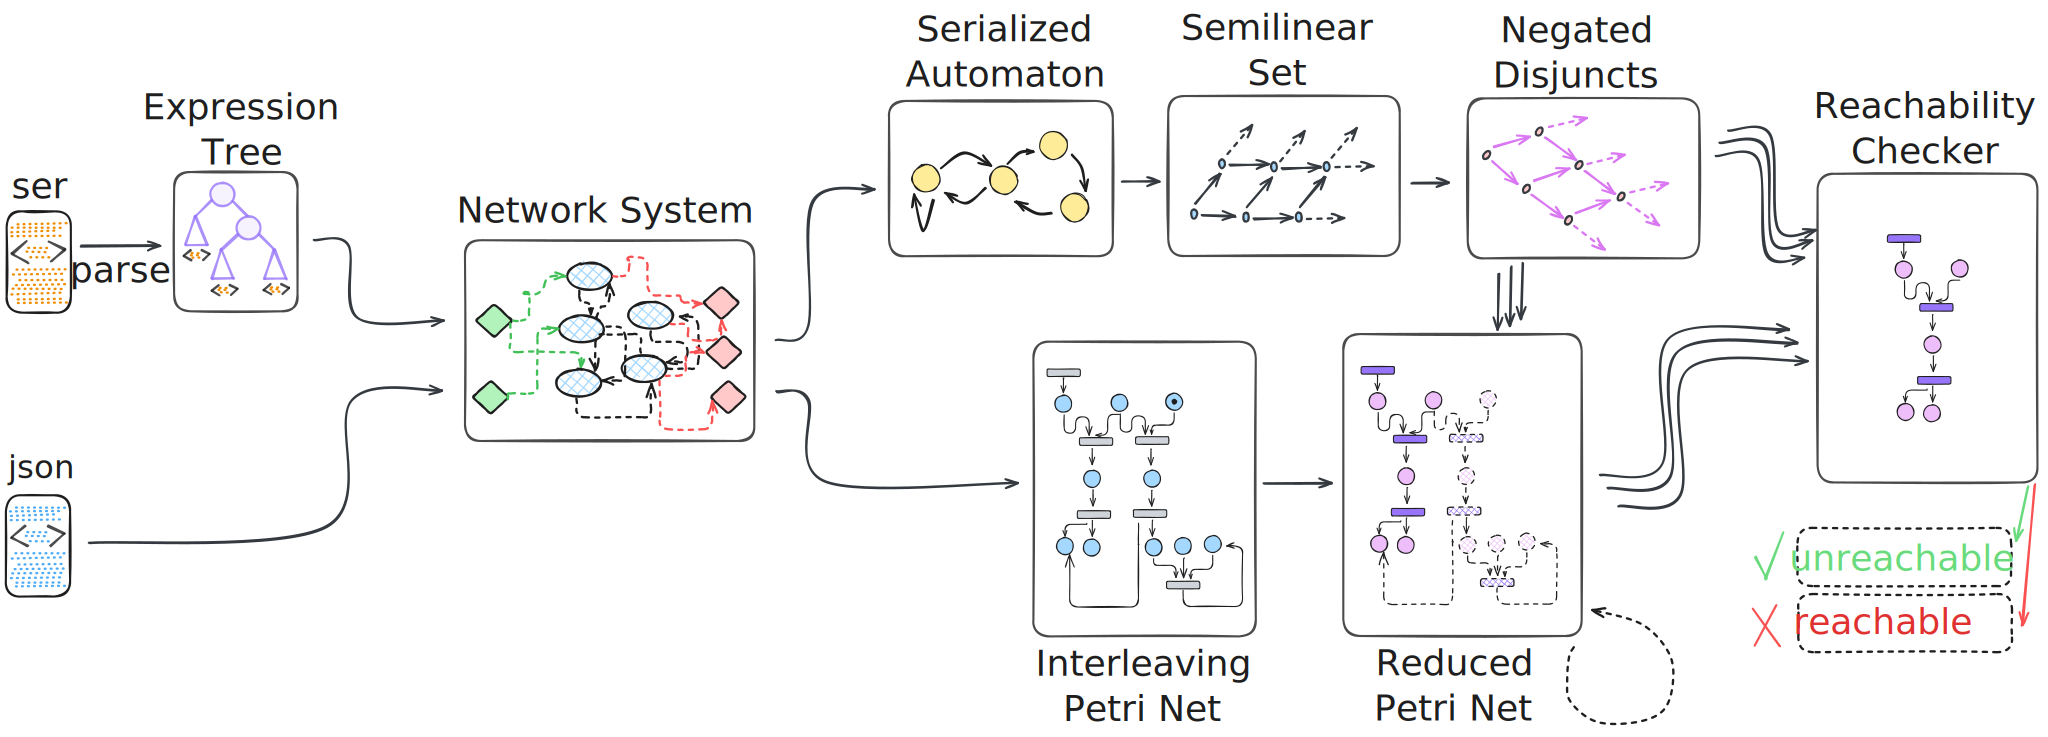
\includegraphics[width=1.0\textwidth]{plots/full_program_flow.pdf}
	\caption{Full program flow. If the program is unreachable --- a serializability proof is produced; otherwise, if it is reachable --- a counterexample trace is generated.}
	\label{fig:full_program_flow}
\end{figure}


\subsection{Optimizations}

\paragraph{Bidirectional Pruning of the Petri Net}
Before any heavy symbolic reasoning takes place, we apply a bidirectional reachability filter to the underlying Petri net.  In the forward pass, we traverse from the initial marking to identify all places and transitions that could ever fire; in the backward pass, we traverse backward from any place that can influence a target constraint.  By intersecting these two reachable sets, we remove every component of the net that cannot both originate and contribute to a solution.  This dramatically shrinks the net in practice, often converting an intractably large model into one small enough for exhaustive analysis.

\paragraph{Redundant‐Constraint Elimination}
When manipulating Presburger sets or their semilinear representations, it is common for some inequalities or disjuncts to add no new coverage beyond what other constraints already guarantee.  The redundant‐constraint elimination pass inspects each linear inequality and each disjunct in a disjunctive normal form, testing whether it is implied by the rest.  Any constraint or disjunct found redundant is dropped, ensuring that subsequent intersection, union, and projection operations work on the smallest necessary formula.  This streamlines the logic formula and prevents exponential blow‐up of case distinctions during solver invocations.

\paragraph{Generate‐Less Constraint Generation}
During set‐construction—especially when introducing new existentially‐quantified variables or combining transition effects—we selectively avoid generating any marking that would strictly dominate an already‐seen solution.  In effect, whenever a candidate disjunct would yield a superset of an existing one, it is skipped entirely.  This “generate‐less” heuristic stops the proliferation of large, overlapping regions in the semilinear description, trading off completeness of intermediate case‐enumeration for concise final representations.  In benchmarks with large state‐spaces, it can reduce the number of intermediate branches by orders of magnitude.

\paragraph{Smart Kleene‐Star Expansion Order}
Expanding Kleene closures (the “\(\mathsf{*}\)” operator) can blow up expressions if done naively in a fixed left‐to‐right order.  Instead, we analyze the structure of subexpressions under the Kleene operator—estimating their branching factor and likely convergence speed—and reorder them so that simpler, low‐branching components are expanded first.  This adaptive ordering often leads to early detection of fixed points or dead‐ends, preventing the combinatorial explosion that arises when complex loops are expanded prematurely.  The net effect is a much more controlled expansion process, improving both time and memory usage on challenging examples.


\begin{figure}[htbp]
	\centering
	
	% Top row: (a), (b), (f)
	\begin{subfigure}[b]{0.45\textwidth}
		\centering
		\includegraphics[width=\textwidth]{plots/bidirectional_pruning_step_a_init.pdf}
		\caption{Step 0: initial petri net, before pruning.}\label{fig:step:a}
	\end{subfigure}\hfill
	\begin{subfigure}[b]{0.45\textwidth}
		\centering
		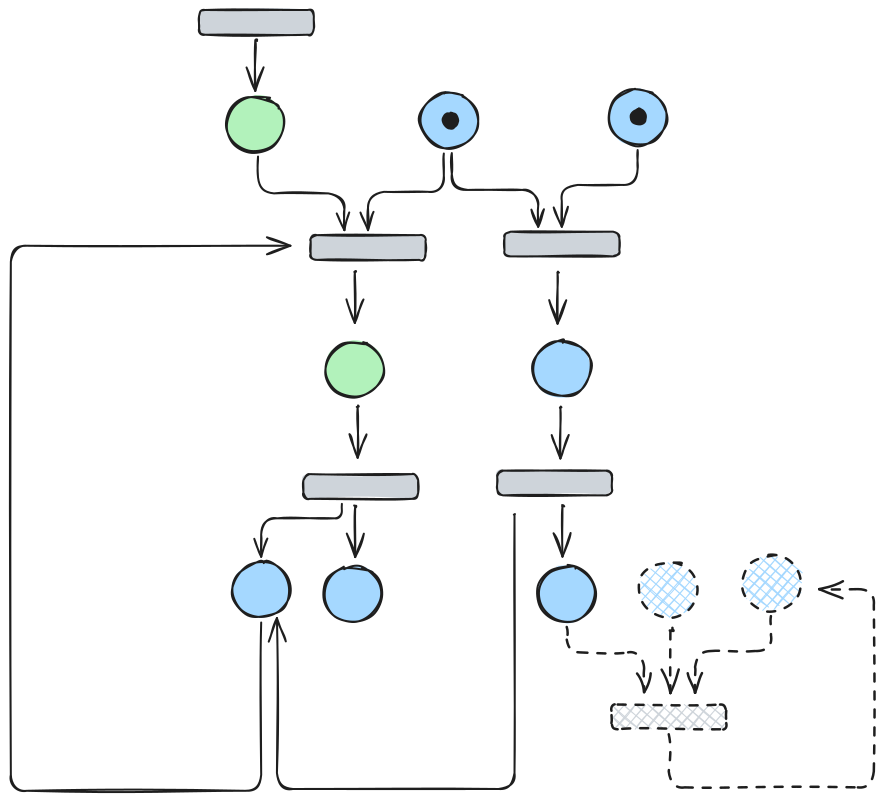
\includegraphics[width=\textwidth]{plots/bidirectional_pruning_step_b_forward.pdf}
		\caption{Step 1: during forward pass.}\label{fig:step:b}
	\end{subfigure}\hfill
	
	
	\vspace{1em}
	
	% Bottom row: (c), (d), then stacked (e)/(f) slot
	\begin{subfigure}[b]{0.30\textwidth}
		\centering
		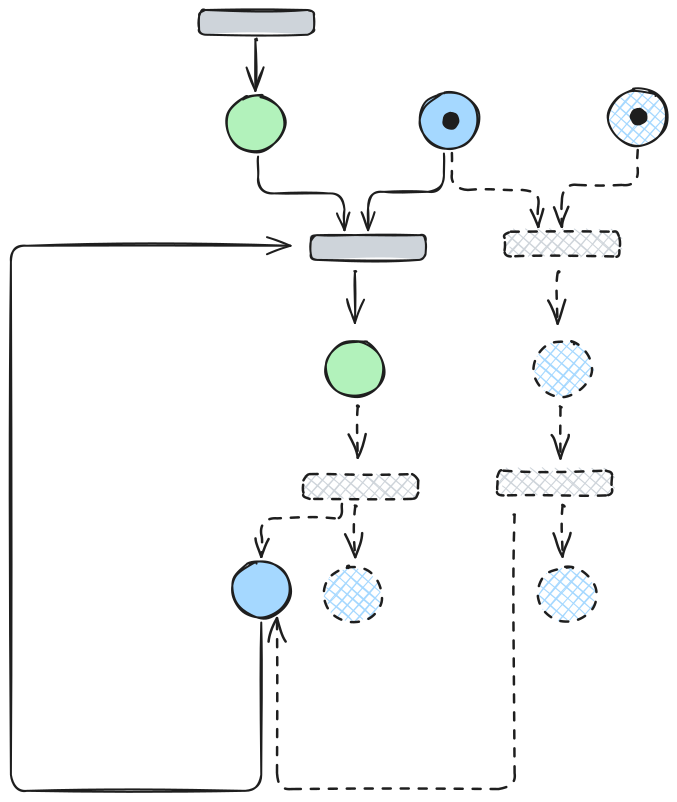
\includegraphics[width=\textwidth]{plots/bidirectional_pruning_step_c_backward.pdf}
		\caption{Step 3: after forward pass, and during backward pass.}\label{fig:step:c}
	\end{subfigure}\hfill
	\begin{subfigure}[b]{0.23\textwidth}
		\centering
		\includegraphics[width=\textwidth]{plots/bidirectional_pruning_step_d_forward.pdf}
		\caption{Step 4: after backward pass, and during forward pass.}\label{fig:step:d}
	\end{subfigure}\hfill
	\begin{subfigure}[b]{0.23\textwidth}
		\centering
		% nested for (e)
		\begin{subfigure}[b]{\textwidth}
		\includegraphics[width=0.5\textwidth]{plots/bidirectional_pruning_step_e_backward.pdf}
			%	       \vspace{-0.5ex}  
%			\raisebox{17ex}{%
%				\includegraphics[width=0.65\textwidth]{plots/bidirectional_pruning_step_e_backward.pdf}%
%			}
			%		\captionsetup{skip=-15.5ex}
			\caption{Step 5: after forward pass, and during backward pass.}\label{fig:step:e}
		\end{subfigure}
		
		\vspace{0.5em}
		
		% nested for (f)
		\begin{subfigure}[b]{\textwidth}
			\centering
			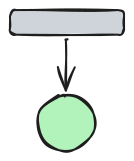
\includegraphics[width=0.23\textwidth]{plots/bidirectional_pruning_step_f_final.pdf}
			\caption{Step 6: final petri net.}\label{fig:step:f:bottom}
		\end{subfigure}
	\end{subfigure}
	
	\caption{A Petri Net after four iterations of bidirectional pruning: two forward passes and two backward passes. Black dots represent initial token markings; green places represent places that are allowed to be reachable in our constraints. Dashed shapes represent places and transitions that are identified as removable in the current iteration, and will be removed after it ends.}
	\label{fig:bidirectional_pruning}
\end{figure}




\newpage
\section{Evaluation}
\label{sec:evaluation}

\begin{enumerate}
    \item Benchmarks (describe our benchmarks)
    \item Results (total time, split out SMPT time from our rust code time)
    \item Analysis of optimizations (how much time they save, petri net sizes, semilinear set sizes)
    \item Limitations (examples we cannot solve, future work that would help)
\end{enumerate}


\subsection{Benchmarks Overview}
\label{subsec:benchmarks}

\begin{itemize}
	\item \textbf{Core expressions \& operators}: Benchmarks testing arithmetic, boolean, and simple control expressions.
	\item \textbf{Fred (mixed arithmetic)}: Mixed control and arithmetic transformations (Fred series).
	\item \textbf{Stop (circular-increment) series}: Circular increment loops and variants.
	\item \textbf{Concurrency \& locking loops}: Concurrent looping patterns with locking and tricky interactions.
	\item \textbf{Non-deterministic choice \& randomness}: Random choice and non-deterministic branching benchmarks.
	\item \textbf{Networking \& system protocols}: Networking protocols and system-level monitoring.
	\item \textbf{Multi-request workflows}: Benchmarks modelling multiple requests or sequential interactions.
	\item \textbf{JSON state-machine examples}: Example JSON-encoded state machine workflows.
\end{itemize}


\subsection{Results}

\begin{table}[ht]
	\centering
	\small
	\setlength{\tabcolsep}{3pt}
	\renewcommand{\arraystretch}{0.9}
	\begin{tabular*}{\textwidth}{@{\extracolsep{\fill}}%
      p{1.3cm}  % Category
	p{3cm}    % Benchmark
			cccc      % Features
			rr        % Runtime
			c         % Serializable
		}
		\toprule
		\textbf{Category}
		& \textbf{Benchmark}
		& \multicolumn{4}{c}{\textbf{Features}}
		& \multicolumn{2}{c}{\textbf{Runtime (ms)}}
		& \textbf{Serializable} \\
		\cmidrule(lr){3-6} \cmidrule(lr){7-8}
		& 
		& \textbf{If}
		& \textbf{While}
		& \textbf{?}
		& \textbf{Yield}
		& \textbf{w/ SMPT}
		& \textbf{w/o SMPT}
		&  \\ 
		\midrule
		
		\multirow{18}{=}{Core expressions \& operators}
		& \texttt{arithmetic.ser}        &  &  &  & \cmark & -- & -- & \cmark \\
		& \texttt{boolean\_ops.ser}      & \cmark &  &  & \cmark & -- & -- & \cmark \\
		& \texttt{seq\_expr.ser}         &  &  &  & \cmark & -- & -- & \cmark \\
		& \texttt{multiple\_vars.ser}    &  &  &  &       & -- & -- & \cmark \\
		& \texttt{mixed\_expr.ser}       & \cmark &  &  &       & -- & -- & \cmark \\
		& \texttt{complex\_expr.ser}     & \cmark &  &  &       & -- & -- & \cmark \\
		& \texttt{if\_expr.ser}          & \cmark &  &  &       & -- & -- & \cmark \\
		& \texttt{while\_expr.ser}       &  & \cmark &  &       & -- & -- & \cmark \\
		& \texttt{if\_while.ser}         & \cmark & \cmark &  & \cmark & -- & -- & \cmark \\
		& \texttt{nested\_while.ser}     &  & \cmark &  &       & -- & -- & \cmark \\
		& \texttt{ex.ser}                &  & \cmark &  & \cmark & -- & -- & \cmark \\
		& \texttt{simple\_assign.ser}    &  &  &  &       & -- & -- & \cmark \\
		& \texttt{yield\_expr.ser}       &  &  &  & \cmark & -- & -- & \cmark \\
		& \texttt{equality\_check.ser}   & \cmark &  &  &       & -- & -- & \cmark \\
		& \texttt{globals.ser}           & \cmark &  &  & \cmark & -- & -- & \cmark \\
		& \texttt{with\_comments.ser}    &  &  &  & \cmark & -- & -- & \cmark \\
		& \texttt{simple\_nonser2.ser}   &  &  &  &       & -- & -- &  \\
		& \texttt{simple\_nonser2\_minus\_yields\_is\_ser.ser} 
		&  &  &  &       & -- & -- &  \\
		\midrule
		
		\multirow{10}{=}{Fred (mixed arithmetic)}
		& \texttt{fred.ser}                 & \cmark & \cmark &  & \cmark & -- & -- & \cmark \\
		& \texttt{fred2.ser}                & \cmark & \cmark &  & \cmark & -- & -- & \cmark \\
		& \texttt{fred2\_arith.ser}         &  & \cmark &  & \cmark & -- & -- & \cmark \\
		& \texttt{fred\_arith.ser}          &  & \cmark &  & \cmark & -- & -- & \cmark \\
		& \texttt{fred\_arith\_simplified\_until\_1.ser}
		&  & \cmark &  & \cmark & -- & -- & \cmark \\
		& \texttt{fred\_arith\_simplified\_until\_2.ser}
		&  & \cmark &  & \cmark & -- & -- & \cmark \\
		& \texttt{fred\_arith\_tricky.ser}   &  & \cmark &  & \cmark & -- & -- & \cmark \\
		& \texttt{fred\_arith\_tricky2.ser}  &  & \cmark &  & \cmark & -- & -- & \cmark \\
		& \texttt{fred\_arith\_tricky3.ser}  &  & \cmark &  & \cmark & -- & -- & \cmark \\
		& \texttt{incrdecr.ser}              &  & \cmark &  &       & -- & -- & \cmark \\
		\midrule
		
		\multirow{7}{=}{Stop (circular-increment) series}
		& \texttt{stop.ser}   &  & \cmark &  &       & -- & -- & \cmark \\
		& \texttt{stop2.ser}  &  & \cmark &  &       & -- & -- & \cmark \\
		& \texttt{stop3.ser}  &  &  &  &       & -- & -- & \cmark \\
		& \texttt{stop3a.ser} &  &  &  &       & -- & -- & \cmark \\
		& \texttt{stop4.ser}  &  & \cmark &  &       & -- & -- & \cmark \\
		& \texttt{stop4a.ser} &  & \cmark &  &       & -- & -- & \cmark \\
		& \texttt{funny.ser}  &  &  &  & \cmark & -- & -- & \cmark \\
		\midrule
		
		\multirow{6}{=}{Concurrency \& locking loops}
		& \texttt{tricky2.ser}                   &  &  &  &       & -- & -- & \cmark \\
		& \texttt{tricky3.ser}                   &  &  &  &       & -- & -- & \cmark \\
		& \texttt{tricky3\_ser.ser}              &  &  &  &       & -- & -- & \cmark \\
		& \texttt{self\_loop.ser}                & \cmark & \cmark &  & \cmark & -- & -- & \cmark \\
		& \texttt{self\_loop2.ser}               & \cmark & \cmark &  & \cmark & -- & -- & \cmark \\
		& \texttt{simple\_nonser2\_turned\_ser\_with\_locks.ser}
		&  &  &  &       & -- & -- &  \\
		\midrule
		
		\multirow{8}{=}{Non-deterministic choice \& randomness}
		& \texttt{nondet.ser}           &  &  & \cmark &       & -- & -- & \cmark \\
		& \texttt{nondet2.ser}          &  &  & \cmark &       & -- & -- & \cmark \\
		& \texttt{nondet\_impl.ser}     &  &  & \cmark &       & -- & -- & \cmark \\
		& \texttt{nondet\_impl2.ser}    &  &  & \cmark & \cmark & -- & -- & \cmark \\
		& \texttt{modulo\_nonser.ser}   &  &  & \cmark &       & -- & -- &  \\
		& \texttt{simple\_nonser3.ser}  &  &  &  &       & -- & -- &  \\
		& \texttt{flag\_non\_ser.ser}   &  &  & \cmark &       & -- & -- &  \\
		& \texttt{flag\_non\_ser\_turned\_ser.ser}
		&  &  & \cmark &       & -- & -- &  \\
		\midrule
		
		\multirow{4}{=}{Networking \& system protocols}
		& \texttt{BGP\_routing.ser}              
		& \cmark & \cmark & \cmark & \cmark & -- & -- & \cmark \\
		& \texttt{snapshot\_isolation\_network\_monitoring.ser}
		& \cmark & \cmark & \cmark & \cmark & -- & -- & \cmark \\
		& \texttt{stateful\_firewall.ser}        
		& \cmark &  & \cmark & \cmark & -- & -- & \cmark \\
		& \texttt{stateful\_firewall\_without\_yields.ser}
		& \cmark &  & \cmark &       & -- & -- & \cmark \\
		\midrule
		
		\multirow{4}{=}{Multi-request workflows}
		& \texttt{multiple\_requests.ser} &  &  &  &       & -- & -- & \cmark \\
		& \texttt{less\_simple\_ser.ser}  &  & \cmark &  & \cmark & -- & -- &  \\
		& \texttt{simple\_nonser.ser}     &  &  &  &       & -- & -- &  \\
		& \texttt{simple\_ser.ser}        &  &  &  & \cmark & -- & -- & \cmark \\
		\midrule
		
		\multirow{4}{=}{JSON state-machine examples}
		& \texttt{data\_flow.json}         &  &  &  &       & -- & -- &  \\
		& \texttt{shopping\_cart.json}     &  &  &  &       & -- & -- &  \\
		& \texttt{login\_flow.json}        &  &  &  &       & -- & -- &  \\
		& \texttt{state\_machine.json}     &  &  &  &       & -- & -- &  \\
		\bottomrule
	\end{tabular*}
	\caption{Overview of all benchmarks by category, features, runtime, and serializability.}
	\label{tab:benchmarks}
\end{table}


\begin{table}[ht]
	\centering
	\resizebox{\textwidth}{!}{%
		\begin{tabular}{%
				l   % Category
				l   % Benchmark
				p{5cm}   % Description
				cccc  % Features: If, While, ?, Yield
				rr    % Runtime: w/ SMPT, w/o SMPT
				c     % Serializable
			}
			\toprule
			\textbf{Category}
			& \textbf{Benchmark}
			& \textbf{Description}
			& \multicolumn{4}{c}{\textbf{Features}}
			& \multicolumn{2}{c}{\textbf{Runtime (ms)}}
			& \textbf{Serializable} \\
			\cmidrule(lr){4-7} \cmidrule(lr){8-9}
			& 
			& 
			& \textbf{If}
			& \textbf{While}
			& \textbf{?}
			& \textbf{Yield}
			& \textbf{w/ SMPT}
			& \textbf{w/o SMPT}
			&  \\
			\midrule
			
			%% Cluster 1: Core expressions & operators
			\multirow{18}{*}{Core expressions \& operators}
			& \texttt{arithmetic.ser}
			& \multirow{18}{5cm}{Benchmarks testing arithmetic, boolean, and simple control expressions}
			&  &  &  & \cmark & -- & -- & \cmark \\
			& \texttt{boolean\_ops.ser}
			& 
			& \cmark &  &  & \cmark & -- & -- & \cmark \\
			& \texttt{seq\_expr.ser}
			& 
			&  &  &  & \cmark & -- & -- & \cmark \\
			& \texttt{multiple\_vars.ser}
			& 
			&  &  &  &  & -- & -- & \cmark \\
			& \texttt{mixed\_expr.ser}
			& 
			& \cmark &  &  &  & -- & -- & \cmark \\
			& \texttt{complex\_expr.ser}
			& 
			& \cmark &  &  &  & -- & -- & \cmark \\
			& \texttt{if\_expr.ser}
			& 
			& \cmark &  &  &  & -- & -- & \cmark \\
			& \texttt{while\_expr.ser}
			& 
			&  & \cmark &  &  & -- & -- & \cmark \\
			& \texttt{if\_while.ser}
			& 
			& \cmark & \cmark &  & \cmark & -- & -- & \cmark \\
			& \texttt{nested\_while.ser}
			& 
			&  & \cmark &  &  & -- & -- & \cmark \\
			& \texttt{ex.ser}
			& 
			&  & \cmark &  & \cmark & -- & -- & \cmark \\
			& \texttt{simple\_assign.ser}
			& 
			&  &  &  &  & -- & -- & \cmark \\
			& \texttt{yield\_expr.ser}
			& 
			&  &  &  & \cmark & -- & -- & \cmark \\
			& \texttt{equality\_check.ser}
			& 
			& \cmark &  &  &  & -- & -- & \cmark \\
			& \texttt{globals.ser}
			& 
			& \cmark &  &  & \cmark & -- & -- & \cmark \\
			& \texttt{with\_comments.ser}
			& 
			&  &  &  & \cmark & -- & -- & \cmark \\
			& \texttt{simple\_nonser2.ser}
			& 
			&  &  &  &  & -- & -- &  \\
			& \texttt{simple\_nonser2\_minus\_yields\_is\_ser.ser}
			& 
			&  &  &  &  & -- & -- &  \\
			\midrule
			
			%% Cluster 2: Fred (mixed arithmetic)
			\multirow{10}{*}{Fred (mixed arithmetic)}
			& \texttt{fred.ser}
			& \multirow{10}{5cm}{Mixed control and arithmetic transformations (Fred series)}
			& \cmark & \cmark &  & \cmark & -- & -- & \cmark \\
			& \texttt{fred2.ser}
			& 
			& \cmark & \cmark &  & \cmark & -- & -- & \cmark \\
			& \texttt{fred2\_arith.ser}
			& 
			&  & \cmark &  & \cmark & -- & -- & \cmark \\
			& \texttt{fred\_arith.ser}
			& 
			&  & \cmark &  & \cmark & -- & -- & \cmark \\
			& \texttt{fred\_arith\_simplified\_until\_1.ser}
			& 
			&  & \cmark &  & \cmark & -- & -- & \cmark \\
			& \texttt{fred\_arith\_simplified\_until\_2.ser}
			& 
			&  & \cmark &  & \cmark & -- & -- & \cmark \\
			& \texttt{fred\_arith\_tricky.ser}
			& 
			&  & \cmark &  & \cmark & -- & -- & \cmark \\
			& \texttt{fred\_arith\_tricky2.ser}
			& 
			&  & \cmark &  & \cmark & -- & -- & \cmark \\
			& \texttt{fred\_arith\_tricky3.ser}
			& 
			&  & \cmark &  & \cmark & -- & -- & \cmark \\
			& \texttt{incrdecr.ser}
			& 
			&  & \cmark &  &  & -- & -- & \cmark \\
			\midrule
			
			%% Cluster 3: Stop (circular-increment) series
			\multirow{7}{*}{Stop (circular-increment) series}
			& \texttt{stop.ser}
			& \multirow{7}{5cm}{Circular increment loops and variants}
			&  & \cmark &  &  & -- & -- & \cmark \\
			& \texttt{stop2.ser}
			& 
			&  & \cmark &  &  & -- & -- & \cmark \\
			& \texttt{stop3.ser}
			& 
			&  &  &  &  & -- & -- & \cmark \\
			& \texttt{stop3a.ser}
			& 
			&  &  &  &  & -- & -- & \cmark \\
			& \texttt{stop4.ser}
			& 
			&  & \cmark &  &  & -- & -- & \cmark \\
			& \texttt{stop4a.ser}
			& 
			&  & \cmark &  &  & -- & -- & \cmark \\
			& \texttt{funny.ser}
			& 
			&  &  &  & \cmark & -- & -- & \cmark \\
			\midrule
			
			%% Cluster 4: Concurrency & locking loops
			\multirow{6}{*}{Concurrency \& locking loops}
			& \texttt{tricky2.ser}
			& \multirow{6}{5cm}{Concurrent looping patterns with locking and tricky interactions}
			&  &  &  &  & -- & -- & \cmark \\
			& \texttt{tricky3.ser}
			& 
			&  &  &  &  & -- & -- & \cmark \\
			& \texttt{tricky3\_ser.ser}
			& 
			&  &  &  &  & -- & -- & \cmark \\
			& \texttt{self\_loop.ser}
			& 
			& \cmark & \cmark &  & \cmark & -- & -- & \cmark \\
			& \texttt{self\_loop2.ser}
			& 
			& \cmark & \cmark &  & \cmark & -- & -- & \cmark \\
			& \texttt{simple\_nonser2\_turned\_ser\_with\_locks.ser}
			& 
			&  &  &  &  & -- & -- &  \\
			\midrule
			
			%% Cluster 5: Non-deterministic choice & randomness
			\multirow{8}{*}{Non-deterministic choice \& randomness}
			& \texttt{nondet.ser}
			& \multirow{8}{5cm}{Random choice and non-deterministic branching benchmarks}
			&  &  & \cmark &  & -- & -- & \cmark \\
			& \texttt{nondet2.ser}
			& 
			&  &  & \cmark &  & -- & -- & \cmark \\
			& \texttt{nondet\_impl.ser}
			& 
			&  &  & \cmark &  & -- & -- & \cmark \\
			& \texttt{nondet\_impl2.ser}
			& 
			&  &  & \cmark & \cmark & -- & -- & \cmark \\
			& \texttt{modulo\_nonser.ser}
			& 
			&  &  & \cmark &  & -- & -- &  \\
			& \texttt{simple\_nonser3.ser}
			& 
			&  &  &  &  & -- & -- &  \\
			& \texttt{flag\_non\_ser.ser}
			& 
			&  &  & \cmark &  & -- & -- &  \\
			& \texttt{flag\_non\_ser\_turned\_ser.ser}
			& 
			&  &  & \cmark &  & -- & -- &  \\
			\midrule
			
			%% Cluster 6: Networking & system protocols
			\multirow{4}{*}{Networking \& system protocols}
			& \texttt{BGP\_routing.ser}
			& \multirow{4}{5cm}{Networking protocols and system-level monitoring}
			& \cmark & \cmark & \cmark & \cmark & -- & -- & \cmark \\
			& \texttt{snapshot\_isolation\_network\_monitoring.ser}
			& 
			& \cmark & \cmark & \cmark & \cmark & -- & -- & \cmark \\
			& \texttt{stateful\_firewall.ser}
			& 
			& \cmark &  & \cmark & \cmark & -- & -- & \cmark \\
			& \texttt{stateful\_firewall\_without\_yields.ser}
			& 
			& \cmark &  & \cmark &  & -- & -- & \cmark \\
			\midrule
			
			%% Cluster 7: Multi-request workflows
			\multirow{4}{*}{Multi-request workflows}
			& \texttt{multiple\_requests.ser}
			& \multirow{4}{5cm}{Benchmarks modelling multiple requests or sequential interactions}
			&  &  &  &  & -- & -- & \cmark \\
			& \texttt{less\_simple\_ser.ser}
			& 
			&  & \cmark &  & \cmark & -- & -- &  \\
			& \texttt{simple\_nonser.ser}
			& 
			&  &  &  &  & -- & -- &  \\
			& \texttt{simple\_ser.ser}
			& 
			&  &  &  & \cmark & -- & -- & \cmark \\
			\midrule
			
			%% Cluster 8: JSON state-machine examples
			\multirow{4}{*}{JSON state-machine examples}
			& \texttt{data\_flow.json}
			& \multirow{4}{5cm}{Example JSON-encoded state machine workflows}
			&  &  &  &  & -- & -- &  \\
			& \texttt{shopping\_cart.json}
			& 
			&  &  &  &  & -- & -- &  \\
			& \texttt{login\_flow.json}
			& 
			&  &  &  &  & -- & -- &  \\
			& \texttt{state\_machine.json}
			& 
			&  &  &  &  & -- & -- &  \\
			
			\bottomrule
		\end{tabular}%
	}
	\caption{Overview of all benchmarks by category, features, runtime, and serializability.}
	\label{tab:benchmarks}
\end{table}

\subsection{Optimization Analysis}


\begin{figure}[htbp]
	\centering
	\includegraphics[width=0.4\textwidth]{plots/petri_size_reduction_plot.pdf}
	\caption{Size reduction of Petri nets through optimization techniques. The plot shows the reduction in the number of places and transitions after applying our optimization passes. Averaged on all Petri Nets of 50 benchmarks (timeout 30 seconds).}
	\label{fig:petri_size_reduction}
\end{figure}


	
\begin{tabular}{l c c c c}
	\toprule
	& \multicolumn{2}{c}{num components} & \multicolumn{2}{c}{periods per component} \\
	\cmidrule(lr){2-3} \cmidrule(lr){4-5}
	& mean & max & mean & max \\
	\midrule
	baseline (all optimizations)    &  3.28 (+0\%) &  22.00 (+0\%) & 1.36 (+0\%) &  4.00 (+0\%) \\
	baseline - remove\_redundant & 10.24 (+6.97\%) & 194 (+172\%)& \textbf{1.79 (+0.43\%)} & 11 (+7\%) \\
	baseline - generate\_less    &\textbf{782.38 (+779.10\%)}&\textbf{20484 (+20462\%)}&1.65 (+0.29\%)& \textbf{15 (+11\%)} \\
	baseline - smart\_order      &  3.36 (+0.09\%) &  22.00 (+0\%) & 1.38 (+0.02\%) &  4.00 (+0\%) \\
	\bottomrule
\end{tabular}
\textbf{The Table compares experiment running with a 30 second timeout}

\newpage
\section{Related Work}
\label{sec:relatedWork}

Related Work includes...


Serializability first introduced by Eswaran et al.~\cite{EsGrKoTr76}.  It is the first to put forth serializability as a correctness condition for concurrent transaction execution.
The paper also covers conflict serializability. 
%
Papadimitriou~\cite{Pa79} proved that even deciding the history of a single interleaving is serializable is NP-hard.

conflict serializability is enforced during runtime in 
with with pessimistic locking approaches (e.g, 2-Phase locking~\cite{BeHaGo87}), or with optimistic locking approaches (e.g., Optimistic Concurrency Control (OCC))~\cite{KuRo81, BuMo06}


Alur et al.~\cite{AlMcPe96}... 
cover conflict serializability (not "regular" serializability, which is what we do). Furthermore, a main caveat is that they focus on a bounded number of transactions



continued by~\cite{BoEmEnHa13}.
In the followup paper (Boujjani et al.) - they also cover conflict serializability, but find a stronger result than Alur, based on unbounded transactions. They find an interesting result that although you can have an infinite conflict graph (when having infinite transactions), then you can still decide conflict serializability in the unbounded case by finding a cycle in the graph when it's non (conflict) serializable, and the cycle length surprisingly does not depend on the number of transactions, which is pretty cool. Another point is that they define a VASS (=Petri Net) that represents the interleaving, and their definition for it is similar to our PN. They then modify it to include a conflict cycle. The most relevant part to us in this paper is that it's on an unbounded number of transactions and also, that they represent Int(S) with a VASS that is similar to us. Still, it's not our notion of serializability (and indeed, they have EXPTIME complexity, while we're probably Ackermann complete?).



Another line of work leverages the highly expressive \textit{Logic of Temporal Actions} (TLA)~\cite{La94}. 
%
These work encode
serializability in TLA+~\cite{SoVaVi20, Ho24},...model checkers (such as TLC and Apalache)~\cite{YuMaLa99, KoKuTr19}.
%
TLA+ can indeed encode an infinite number of transactions. For example, here is the TLA+ spec for encoding serializability.
However, for doing model checking on a TLA spec (with the TLC model checker) --- the model checker takes a .cfg file as additional input, in in the .cfg you explicitly specify all of the sets in the model, and these have to be finite. You can see this here where the model checking file needs to encode in advance the number of transactions (see attached figure)



\todo{go over the paper and its citing papers}
Me:
1992 paper today, they seem to model a concurrent execution with petri nets but they don't ask if all executions are serializable which is our subject matter

Furthermore, other work cover additional consistency models, such as causal consistency, which was put forth by Lamport~\cite{La78}, en extended to shared memory systems as \textit{causal memory}~\cite{AhNeBuKoHu95}. (include causal + consistency, designed in COPS~\cite{LlFrKaAn11}). The have been a plethora of works on model checking systems that adhere to causal consistency, and hence the complexity of such procedures~\cite{BoEnGuHa17,ZeBiBoEnEr19,LaBo20}

\todo{go over Mark's notes}



\todo{go over Espinoza complexity results}

Our work also builds upon both theoretical literature, as well as practical results, pertaining to Petri Nets~\cite{Reisig12,Mu89}.
%
In terms of theory, our undecidability result is based on a classic result by Hack~\cite{Ha76}, showing that, given two Petri Nets, it is undecdiable to answer whether they have equivalent reachbility sets. Hack based his result on the work of Rabin (which was never published). These undecdiability results follow from a series of reductions, originating from Hilbert's 10th problem, i.e., deciding if a Diophantine polynomial has an integer root (a problem that was proved undecidable by Matijas{\'e}vi{\v{c}}~\cite{Ma70}).
%
Later, Jan{\v{c}}ar~\cite{Ja95} simplified this proof by using Petri Nets to simulate 2-counter Minsky Machines, which are univerally comptuable and hence undecidable~\cite{Mi67}. Moreover, Jan{\v{c}}ar's result is stronger as it shows that this equality is undecidable even for Petri Nets with five unbounded places~\cite{Ja95}.
%
We refer the reader to a survey by Esparza and Nielsen~\cite{EsNi94} for a comprehensive summary on additional decidability results pertaining to Petri Nets.


Deciding reachaility for Petri Nets:

- Mayr~\cite{Ma81} was the first to put forth an algorithm for deciding reachability for Petri Nets in the unbounded case (note that for a bounded net this is trivial as you can enumerate all reachable markings.)

- This algorithm was later improved and simplified by Kosaraju~\cite{Ko82}, and then by Lambert~\cite{La92}.

- Very recently, the Complexity was recently proven to be Ackermann complete~\cite{CzWo22}, indicating it inherently infeasible in practice to solve on large problems.

These algorithms have inspired various Petri Net reachability tools, such as K-Reach~\cite{DiLa20} and SMPT~\cite{AmDa23}, which employs an SMT-based approach~\cite{AmBeDa21, AmDaHu22} which reduces the reachability problem to a satisfiability query (that is subsequently dispatched to the state-of-the-art Z3 solver~\cite{DeBj08}).

 


\section{Discussion}
\label{sec:discussion}

\subsection{Conclusion}

To the best of our knowledge, ours is the first 
tool capable of verifying serializability in unbounded domains.
%
While these contributions represent significant advances, to our knowledge, our 
work is the first to:
(i) Decide serializability universally --- \textit{considering all executions} 
purely through program semantics and final states, independent of read/write 
conflicts; 
(ii) Support \textit{unbounded} transaction systems; and
(iii) Provide a complete end-to-end implementation.

\todo{Limitations?}
Examples we cannot solve, future work that would help
To conclude..


\subsection{Future Work}
Next..

We plan to use polyhedral reductions~\cite{AmBeDa21} that are structural reduction~\cite{Be87,BeLeDa20} of the form $(N_1, m_1) \vartriangleright_E (N_2, m_2)$, where $(N_1, m_1)$ is the Petri net we want to analyze, $(N_2, m_2)$ is a reduced version of this net (easier to model check), and $E$ is a Presburger formula that permits to reconstruct of the state space of $N_1$ from that of $N_2$. We plan to leverage this mechanism to trace back certificates obtained on the reduced net $N_2$ to the original net $N_1$, that would be the only kind of structural reduction for which such operation is possible.

\todo{Different notions of serializability}
\begin{itemize}
    \item \todo{Current notion: clients independently submit a request and get a response, and later they all get together and see if what they got was serializable}
    \item \todo{Stronger: clients are not independent, or sequentially execute some parts. General: we have some happens-before on the requests/responses}
    \item \todo{Weaker: the clients cannot communicate with each other afterwards to determine whether what they got was serializable, or they can only communicate in a limited way}
    \item \todo{Infinite / unbounded executions}
\end{itemize}


\newpage

\bibliographystyle{ACM-Reference-Format}
\bibliography{references}

\newpage

%% Appendix
\appendix

\section{Additional NS Examples}
\label{appendix:MoreNsExamples}



\subsection{Motivating Examples \#1}
\label{appendix:subsec::Ex1A:NS}


Recall the code snipped from Listing~\ref{lst:MotivatingExample1Ser}:


\begin{minipage}[t]{0.3\textwidth}
	\begin{lstlisting}[caption={Without yield or lock (serializable)}]
	request main: 
		X := 1 
		// no yield
		y := X 
		X := 0
		return y 
	\end{lstlisting}
\end{minipage}

\begin{figure}[H]
	\centering
	\includegraphics[width=0.9\textwidth]{plots/code_1_NS.png}
	\caption{Network System for interleaving executions of Listing~\ref{lst:MotivatingExample1Ser} program.}
	\label{fig:code1ExampleNS}
\end{figure}


\begin{figure}[H]
	\centering
	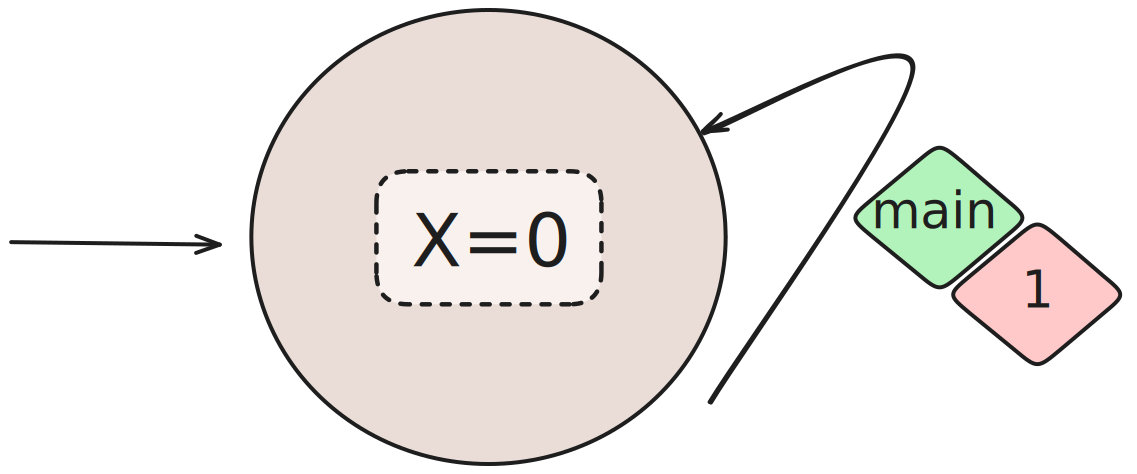
\includegraphics[width=0.35\textwidth]{plots/code_1_NFA.png}
	\caption{NFA for serialized executions of Listing~\ref{lst:MotivatingExample1Ser} program.}
	\label{fig:code1ExampleNFA}
\end{figure}



\begin{figure}[H]
	\centering
	\includegraphics[width=0.6\textwidth]{plots/code_1_PN_with_annotation.png}
	\caption{Petri Net for interleaving executions of Listing~\ref{lst:MotivatingExample1Ser} program.}
	\label{fig:code1ExamplePN}
\end{figure}

%

\subsection{Motivating Examples \#2}
\label{appendix:subsec::Ex1B:NS}

For details, see the main text (Sec.~\ref{sec:problem-definition}).


\subsection{Motivating Examples \#3}
\label{appendix:subsec:Ex1C:NS}

Recall our third motivating example, presented in Listing~\ref{lst:MotivatingExample3SerAgain}.

\begin{minipage}[t]{0.3\textwidth}
	\begin{lstlisting}[caption={With yield and lock (serializable)}]
		request foo: 
			// lock
			while (L == 1): 
				yield
			L := 1 
		
			X := 1
			yield
			y := X 
			X := 0
		
			// unlock    
			L := 0
			return y 
	\end{lstlisting}
\end{minipage}

This program corresponds to the following Network System (NS):

\begin{figure}[htbp]
	\centering
	\includegraphics[width=1.1\textwidth]{plots/code_3_NS.png}
	\caption{Network System for interleaving executions of Listing~\ref{lst:MotivatingExample3Ser} program.}
	\label{fig:code3ExampleNS}
\end{figure}


\begin{figure}[htbp]
	\centering
	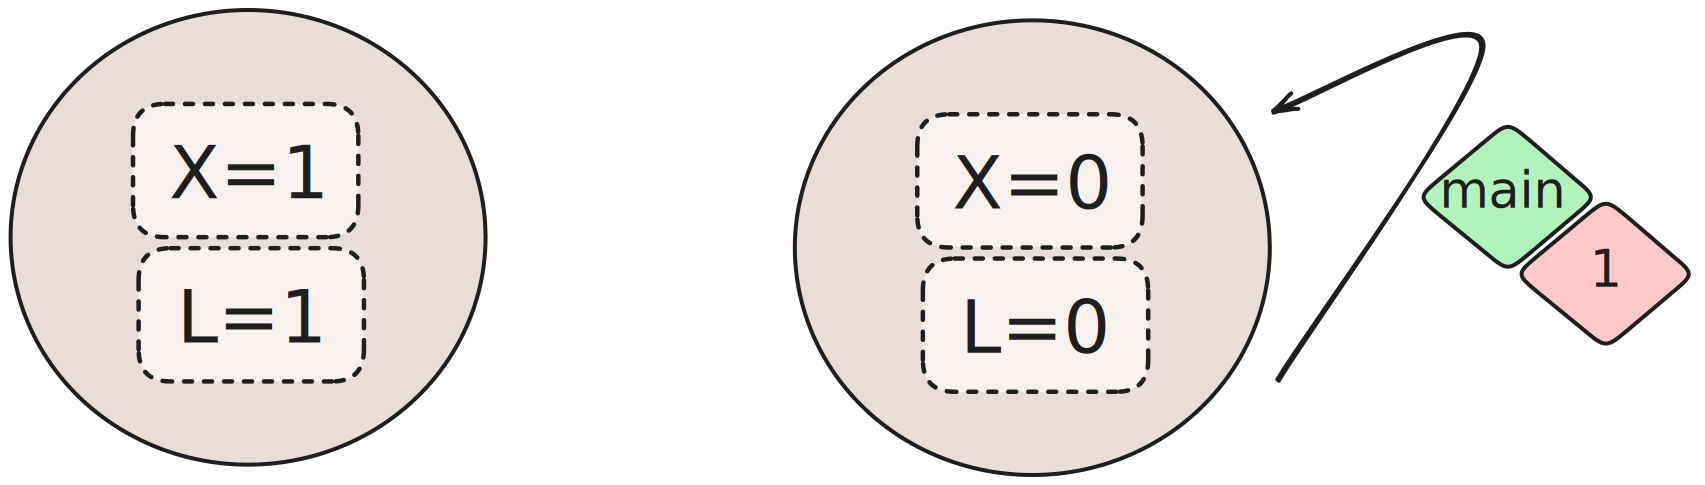
\includegraphics[width=0.4\textwidth]{plots/code_3_NFA.png}
	\caption{NFA for serialized executions of Listing~\ref{lst:MotivatingExample3Ser} program.}
	\label{fig:code3ExampleNFA}
\end{figure}



\begin{figure}[H]
	\centering
	\includegraphics[width=0.8\textwidth]{plots/code_3_PN_with_annotation.png}
	\caption{Petri Net for interleaving executions of Listing~\ref{lst:MotivatingExample3Ser} program.}
	\label{fig:code3ExamplePN}
\end{figure}

\newpage


\section{Motivating Example: Snapshot Isolation}
\label{appendix:snapshotIsolationExample}



The next program is motivated by system monitoring.
The system has two nodes (represented by the global variables $N_1$ and $N_2$) which monitor ongoing traffic in the network, and are originally both active (as indicated by their initial values [$N_1=1,N_2=1$]).
%
The {\color{ForestGreen}$\blacklozenge_\text{main}$} request takes a ``snapshot'' of the system, i.e., locally records the current activation status of each of the two nodes.
%
Subsequently, in the first request, and any future ones in which both nodes are active, each in-flight request thread  non-deterministically decides which of the two nodes to deactivate, i.e. set [$N_i:=0$]. This policy is consistent with real-world settings for maintaining overall energy efficiency.
%
The {\color{ForestGreen}$\blacklozenge_\text{main}$} request eventually returns the current sum of active nodes in the system.
%
In order for the system to emulate multiple iterations, our setting also includes two additional requests, {\color{ForestGreen}$\blacklozenge_\text{activate\_n1}$},{\color{ForestGreen}$\blacklozenge_\text{activate\_n2}$} which activate the nodes $N_1$ and $N_2$, respectively.
%
We note that the program is non-serializable due to the yield operation that appears immediately after the recording (snapshot) of the node activity. One such example for a non-serializable behavior occurs when two {\color{ForestGreen}$\blacklozenge_\text{main}$} requests record two active monitor nodes and yield; Then, having each request turn off the complement node. As a result of each request operating based on its isolated ``snapshot'' of the initial global state, both monitor nodes can be turned off and we can attain a request with {\color{ForestGreen}$\blacklozenge_\text{main}$}/{\color{red}$\blacklozenge_0$} (for [$N_1+N_2=0+0=0$]).
%
We note that in any serializable execution, no two {\color{ForestGreen}$\blacklozenge_\text{main}$} requests can record both monitors as active, and hence, they cannot both have an interleaving in which each separate monitor is deactivated (hence, a response of {\color{red}$\blacklozenge_0$} is unattainable in serializable executions).




\begin{minipage}[t]{1.0\textwidth}
	\begin{lstlisting}[caption={Snapshot-based monitor deactivation (not serializable, as it can return a sum of 0 active monitors)}]
				// initialize both monitors to be active
				N_1_ACTIVE := 1
				N_2_ACTIVE := 1
				
				request main:
					// take snapshot
					n_1_active_snapshot := N_1_ACTIVE
					n_2_active_snapshot := N_2_ACTIVE
					yield
					
					if (n_1_active_snapshot == 1) and (n_2_active_snapshot == 1):
					// if both nodes active --- choose which one to deactivate 
						if (?): 
							  N_1_ACTIVE := 0
						else:
							  N_2_ACTIVE := 0
						
					return N_1_ACTIVE + N_2_ACTIVE  // total active nodes
					
				
				request activate_n1:
					    N_1_ACTIVE := 1
				
				request activate_n2:
					    N_2_ACTIVE := 1
				
				
			\end{lstlisting}
\end{minipage}

%only 0 in non-serializable runs!

%\todo{start}

%/snapshot_isolation_directly_as_NS_with_yields

%\begin{figure}[h]
%	\centering
%	\includegraphics[width=1.0\linewidth]{plots/snapshot\_isolation\_JSON\_with\_yields.pdf}
%	\caption{Snapshot Isolation with Yields.}
%	\label{fig:snapshotIsolationJsonWithYields}
%\end{figure}
%
%
%
%%/snapshot_isolation_directly_as_NS_without_yields
%
%\begin{figure}[h]
%	\centering
%	\includegraphics[width=1.0\linewidth]{plots/snapshot\_isolation\_JSON\_without\_yields.pdf}
%	\caption{Snapshot Isolation without Yields.}
%	\label{fig:snapshotIsolationJsonWithoutYields}
%\end{figure}


%\todo{maybe we have: (1) a copy of the global automaton; (2) a copy of the local automaton (with yields) with coloring of edges that don't exist in the one without yields}


%\begin{figure}[h]
%	\centering
%	\includegraphics[width=0.65\linewidth]{plots/BgpColoredRouting.pdf}
%	\caption{Routing policy in example 7.}
%	\label{fig:pdfimage}
%\end{figure}

%\newpage
%
%
%example – 8
%
%\noindent
%\begin{minipage}[t]{0.45\textwidth}
%	\begin{lstlisting}[caption={foo (serializable)}]
	%	request foo: 
	%	    if (?):
	%	        X := (X + 2) % 3 
	%	        // no yield
	%	        return X
	%	
	%	    else:
	%	        X := (X + 1) % 3
	%	        // no yield
	%	        return X
	%		\end{lstlisting}
%\end{minipage}
%\hfill
%\begin{minipage}[t]{0.45\textwidth}
%\begin{lstlisting}[caption={foo (non serializable)}]
%request foo: 
%     if (?):
%         X := (X + 2) % 3 
%         yield
%         return X
%
%     else:
%         X := (X + 1) % 3
%         yield
%         return X
%	\end{lstlisting}
%\end{minipage}
%
%One output that is attainable only via non-serializable executions is 
%\[
%\{(foo,1),(foo,1),(foo,1),(foo,3)\}
%\]
%
%
%%\newpage
%
%
%example – 9
%
%\noindent
%\begin{minipage}[t]{0.45\textwidth}
%	\begin{lstlisting}[caption={foo (serializable)}]
%request foo:
%    if(STOP == 0):
%        X := (X + 1) % 4
%
%    yield
%
%    if(STOP == 0):
%        X := (X + 1) % 4
%
%        STOP := ?
%        
%        if(STOP == 1):
%	        return X
%        return 0
%	\end{lstlisting}
%\end{minipage}
%\hfill
%\begin{minipage}[t]{0.45\textwidth}
%	\begin{lstlisting}[caption={foo (non serializable)}]
%request foo:
%    if(STOP == 0):
%        X := (X + 1) % 4
%
%    yield
%
%    if(STOP == 0):
%        X := (X + 2) % 4
%
%        STOP := ?
%        
%        if(STOP == 1):
%	        return X
%        return 0
%	\end{lstlisting}
%\end{minipage}





\newpage
%% Appendix
%\appendix

\section{Proof: Bidirectional Optimizatoin Correctness}
\label{appendix:BidirectionalProof}





	\subsection{Preliminaries}
	
	\begin{definition}[Petri Net]
		A \emph{Petri net} is a tuple
		\[
		N = (P,\,T,\,\Pre,\,\Post)
		\]
		where
		\begin{itemize}
			\item $P$ is a finite set of \emph{places},
			\item $T$ is a finite set of \emph{transitions},
			\item $\Pre: P\times T \to \mathbb{N}$ is the \emph{pre-incidence} function,
			\item $\Post: P\times T \to \mathbb{N}$ is the \emph{post-incidence} function.
		\end{itemize}
	\end{definition}
	
	\begin{definition}[Marking]
		A \emph{marking} is a function $M: P \to \mathbb{N}$. We write $M(p)$
		for the number of tokens in place $p$.  The initial marking is
		denoted $M_0$.  A transition $t\in T$ is \emph{enabled} at marking
		$M$ if $\forall p\in P:\,M(p)\ge\Pre(p,t)$.  Firing $t$ yields the
		new marking
		\[
		M' = M - \Pre(\cdot,t) + \Post(\cdot,t),
		\]
		written $M \xrightarrow{t} M'$.
	\end{definition}
	
	\begin{definition}[Firing Sequence]
		A sequence $\sigma = t_1 t_2 \cdots t_k \in T^*$ is \emph{fireable}
		from $M_0$ if there exist markings $M_1,\dots,M_k$ such that
		$M_0\xrightarrow{t_1}M_1\cdots\xrightarrow{t_k}M_k$.  We write
		$M_0 \xrightarrow{\sigma} M_k$.
	\end{definition}
	
	\begin{definition}[Semilinear Target Set]
		A \emph{semilinear} set $T\subseteq \mathbb{N}^P$ is a finite union of
		linear sets.  We assume $T$ is given by a finite description of its
		linear components.  We view $T$ as the \emph{target} set of markings
		we wish to reach.
	\end{definition}
	
	\subsection{The Bidirectional Pruning Algorithm}
	
	Let $N=(P,T,\Pre,\Post)$, initial marking $M_0$, and target set
	$T\subseteq\mathbb{N}^P$ be fixed.
	
	\begin{definition}[Forward Over‐Approximation]
		Define the operator $\mathcal{F}:\mathcal{P}(P\cup T)\to\mathcal{P}(P\cup T)$ by
		\[
		X \mapsto X
		~\cup~
		\{\,t\in T \mid \forall p\in P:\; \Pre(p,t)>0 \implies p\in X\}
		~\cup~
		\{\,p\in P \mid \exists t\in X\cap T,\ \Post(p,t)>0\}.
		\]
		Starting from $X_0 = \{\,p\mid M_0(p)>0\}$, iterate
		$X_{i+1} = \mathcal{F}(X_i)$ until a least fixed‐point
		$X^*=\bigcup_i X_i$ is reached.  Call $X^*_P = X^*\cap P$ the set of
		\emph{forward‐reachable} places.
	\end{definition}
	
	\begin{definition}[Backward Over‐Approximation]
		Let
		\[
		Y_0 = \{\,p\in P \mid \exists M\in T:\;M(p)>0\}
		\]
		be the places unconstrained to zero by the target.  Define
		$\mathcal{B}:\mathcal{P}(P\cup T)\to\mathcal{P}(P\cup T)$ by
		\[
		Y \mapsto Y
		~\cup~
		\{\,t\in T \mid \forall p\in P:\; \Post(p,t)>0 \implies p\in Y\}
		~\cup~
		\{\,p\in P \mid \exists t\in Y\cap T,\ \Pre(p,t)>0\}.
		\]
		Iterate $Y_{i+1} = \mathcal{B}(Y_i)$ until a least fixed‐point
		$Y^*=\bigcup_i Y_i$ is reached.  Call $Y^*_P = Y^*\cap P$ the set of
		\emph{backward‐relevant} places.
	\end{definition}
	
	\begin{definition}[Pruned Net]
		The \emph{pruned} subnet is
		\[
		N' = \bigl(P',\,T',\,\Pre|_{P'\times T'},\,\Post|_{P'\times T'}\bigr)
		\]
		where
		\[
		P' = X^*_P \;\cap\; Y^*_P,
		\quad
		T' = \{\,t\in T \mid
		\forall p:\;\Pre(p,t)>0\implies p\in P',\;
		\forall p:\;\Post(p,t)>0\implies p\in P'
		\}.
		\]
	\end{definition}
	
	\subsection{Invariant and Correctness}
	
	Intuitively, $P'$ contains exactly those places that
	\emph{may} occur in some firing sequence from $M_0$ to a marking in $T$.
	
	\begin{definition}[Witnessable Place]
		A place $p\in P$ is \emph{witnessable} if there exists a firing
		sequence $\sigma\in T^*$ and markings $M$ and $M'$ such that
		\[
		M_0 \xrightarrow{\sigma_1} M
		\quad\text{and}\quad
		M \xrightarrow{\sigma_2} M'
		\quad\text{with}\quad
		M'(p)>0
		\quad\text{and}\quad
		M'\in T.
		\]
		In other words, $p$ can carry a token in some execution from $M_0$ into the target set.
	\end{definition}
	
	\begin{theorem}[Pruning Invariant]
		\label{thm:invariant}
		If a place $p$ is witnessable, then $p\in P'$.  Equivalently, the
		pruned net $N'$ \emph{over‐approximates} the set of witnessable places.
	\end{theorem}
	
	\begin{proof}
		We split the argument into two parts.
		
		\paragraph{(1) Forward‐reachability.}
		Suppose $p$ is witnessable.  Then there is a prefix
		$\sigma_1\in T^*$ such that $M_0\xrightarrow{\sigma_1}M$ and
		$M(p)>0$.  By standard Petri‐net monotonicity, every place that
		receives a token in the course of $\sigma_1$ must appear in the
		forward fixed‐point $X^*_P$.  Hence $p\in X^*_P$.
		
		\paragraph{(2) Backward‐relevance.}
		Again, since $p$ is witnessable, there is a suffix
		$\sigma_2\in T^*$ from $M$ to $M'\in T$ with $M'(p)>0$.  Working
		backwards from $T$, every place that can contribute to satisfying
		semilinear constraints (i.e.\ those places that might be tested
		positive in $T$) appears in the backward fixed‐point $Y^*_P$.  Thus
		$p\in Y^*_P$.
		
		\paragraph{Conclusion.}
		Combining (1) and (2) yields $p\in X^*_P\cap Y^*_P = P'$, as desired.
	\end{proof}
	
	\subsection{Termination and Complexity}
	
	\begin{lemma}
		Each iteration of $\mathcal{F}$ and $\mathcal{B}$ strictly increases
		the set of included elements (unless already at the fixed‐point), and
		the total number of elements is finite.  Hence both reach their
		fixed‐points in at most $|P|+|T|$ iterations each.
	\end{lemma}
	
	\begin{proof}
		Immediate from monotonicity and finiteness.
	\end{proof}
	
	\noindent
	Therefore the bidirectional pruning converges in polynomial time
	(mostly linear in the net‐size per pass), and preserves exactly the
	places and transitions that \emph{may} appear in some execution from
	$M_0$ into $T$.
	


\input{sections/9_appendix_invariant_example}
\input{sections/9_appendix_toy_petri_net.tex}


\section{SMPT}
\label{appendix:smpt}



\texttt{SMPT} (\emph{Satisfiability Modulo Petri Nets}) is a tool incorporating a portfolio of symbolic model checking techniques --- including Bounded Model Checking (BMC)~\cite{BiCiClZh99}, state equation reasoning~\cite{Mu77}, $k$-induction~\cite{ShSiSt20}, Property Directed Reachability (PDR)~\cite{Br11,AmDaHu22}, and random state space exploration. It acts as a front-end to an SMT solver (\texttt{Z3}~\cite{DeBj08} in our setting), while also incorporating domain-specific knowledge from Petri net theory, such as invariants and structural properties. \texttt{SMPT} has participated in the last five editions of the \textit{Model Checking Contest} (MCC), an international competition for model checking tools. In its most recent participation, it achieved a bronze medal and a $100\%$ confidence level score, indicating it never returned an incorrect verdict~\cite{mcc:2025}.

\texttt{SMPT} distinguishes itself from other tools in two ways that are particularly relevant to our setting and motivated its adoption. First, to the best of our knowledge, it is the only model checker for Petri Nets that provides a proof of its verdict, regardless of the underlying verification technique. This means it either produces a witness trace when the property is reachable, or, more interestingly, a certificate of non-reachability~\cite{AmDaHu22} when the property is found to be unreachable.
%
The second distinguishing feature relates to our ongoing work on polyhedral reductions~\cite{AmBeDa21}, as elaborated in Sec.~\ref{sec:discussion}.



%\newpage

\end{document}
